\chapter{DESARROLLO DEL ENFOQUE DE MERCADO.} %(((

% === DESARROLLO DE ENFOQUES === (((
Se llevó a cabo el enfoque de mercado de acuerdo a lo mencionado en el capítulo VI.
Para cada uno de los activos para los que se llevó a cabo este método, se realizó
un modelo de regresión lineal múltiple y se corroboró que la muestra de mercado
cumpliera con los supuestos del modelo para ser estadísticamente significativa.
Esto es, que represente de manera confiable las características del mercado
utilizado. \\[2mm]
A continuación se muestra el desarrollo del enfoque de mercado.
% )))

\section{Tanque para Aire Comprimido.} % (((

\subsection{\centering --- Mercado Utilizado ---} % (((
Se toma la siguiente muestra estadísticamente significativa, y se 
comprueba que lo es, en las siguientes secciones.
\begin{figure}[hbtp!]
	\centering
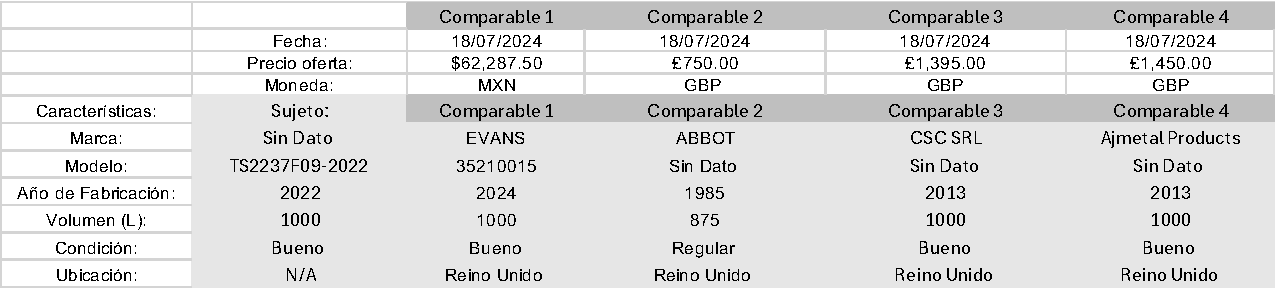
\includegraphics[width= 0.6 \linewidth, page = 1]{../0.imagenes/CAP_8/mercado_1_1}
\end{figure}
\begin{figure}[hbtp!]
	\centering
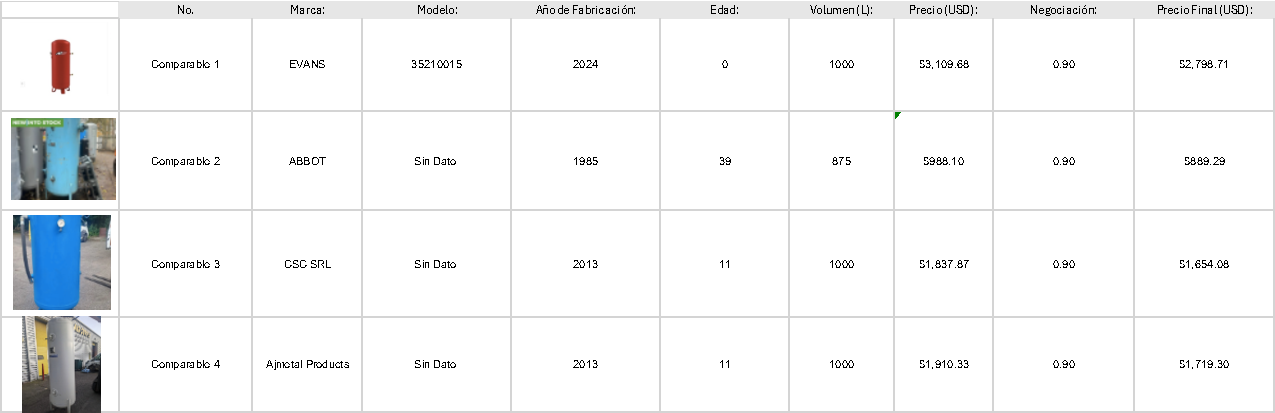
\includegraphics[width= 0.9 \linewidth, page = 1]{../0.imagenes/CAP_8/mercado_1_2}
\end{figure}
% )))

\subsection{\centering --- Variables ---} % (((
\begin{center}
  \begin{tabular}{|l|l|l|}
    \hline 
    Variable & Descripción   & Unidades\\ \hline 
    Y:  & Precio Final del activo  & USD \\ \hline 
    X1: & Edad del activo    & Años \\ \hline 
		X2: & Volumen del activo & \(m ^ 3\) \\ \hline 
  \end{tabular}
\end{center} 
% )))

\subsection{\centering --- Matriz de Dispersion ---} % (((
\begin{center}
  \begin{tabular}{|p{11cm}|p{5cm}|}
    \hline
    Gráfica & Interpretación. \\ \hline 
    \begin{minipage}{\textwidth}
    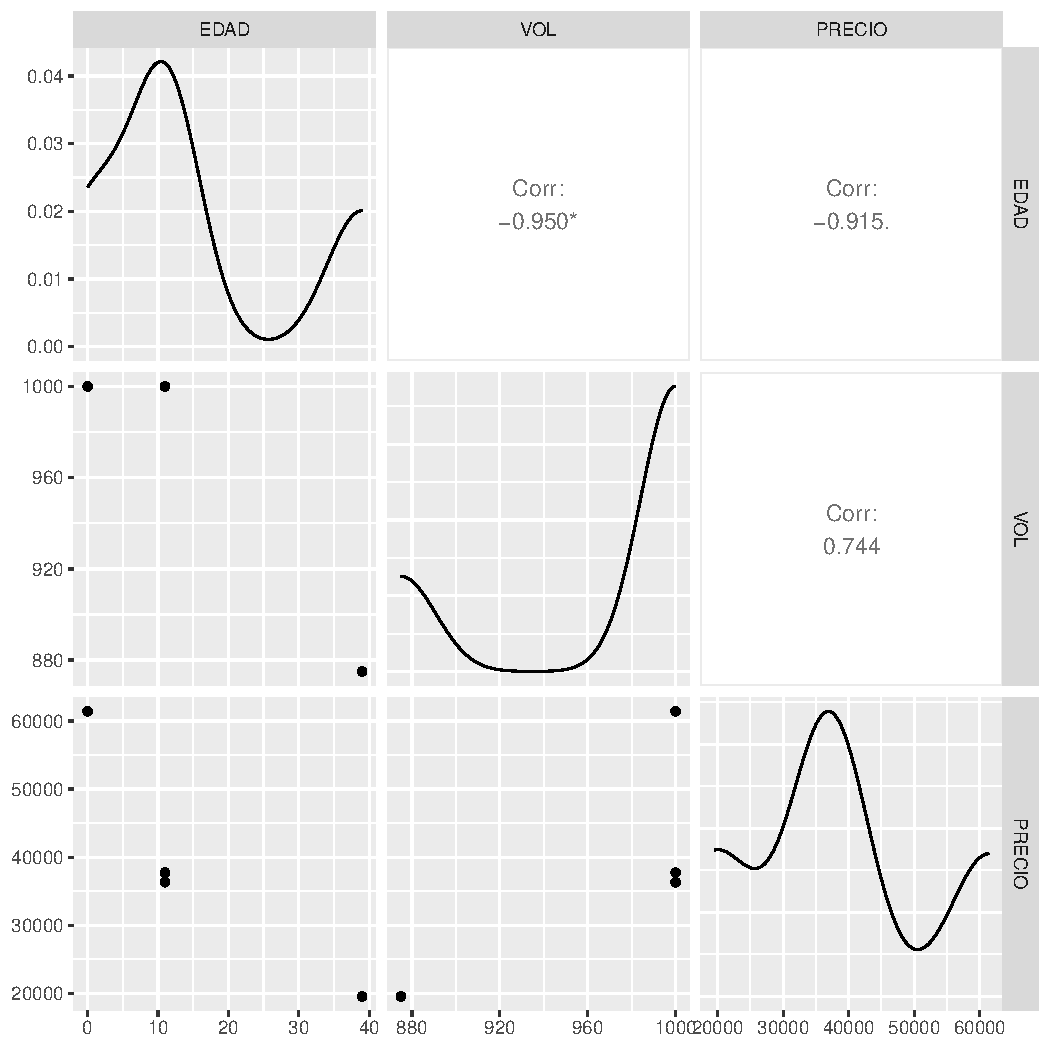
\includegraphics[width= 0.5 \linewidth, page=1]{../0.documentos/3_MERGED_MARKET/1_TANQUE/r/Rplots.pdf}
    \end{minipage} 
    &
		Se tiene una correlación lineal negativa fuerte (el \(91.5\%\) de los datos lo corroboran),
		entre la Edad del Activo, y el Precio del Activo.
		\\ \hline 
  \end{tabular}
\end{center} 
% )))

\subsection{\centering --- Supuestos del Modelo de Regresión ---} % (((

Se realiza el análisis estadístico con un \(90\%\) de confianza. \\ 
Es decir, \(1- \alpha = 0.9\).

\subsubsection{--- Homocedasticidad ---} % (((
\begin{center}
  \begin{tabular}{|l|p{8cm}|}
    \cline{1-2}
    \multicolumn{2}{|c|}{Hipótesis}\\ \cline{1-2}
    \multicolumn{2}{|l|}{\(H_0:\) La varianza de los residuales es constante.} \\ 
    \multicolumn{2}{|l|}{\(H_a:\) La varianza de los residuales no es constante.} \\ \cline{1-2}
    Estadístico de Prueba & \(BP = 4\).\\ \cline{1-2} 
		Región de Rechazo de \(H_0\) & \((0, \alpha )\).\\ \cline{1-2} 
    Valor \(p\) & \(0.1353\).\\ \cline{1-2} 
    Conclusión & Se tiene que \(p> \alpha\). \newline 
		Por tanto no se rechaza \(H_0\). \newline 
		Es decir, la varianza no es constante. \\ \cline{1-2} 
  \end{tabular}
\end{center}
% )))

\subsubsection{--- Independencia ---} % (((
\begin{center}
  \begin{tabular}{|l|p{8cm}|}
    \cline{1-2}
    \multicolumn{2}{|c|}{Hipótesis}\\ \cline{1-2}
    \multicolumn{2}{|l|}{\(H_0:\) Los residuos son independientes.} \\ 
    \multicolumn{2}{|l|}{\(H_a:\) Los residuos no son indpendientes.} \\ \cline{1-2}
    Estadístico de Prueba & \(DW = 2.5\).\\ \cline{1-2} 
		Región de Rechazo de \(H_0\) & \((0, \alpha )\).\\ \cline{1-2} 
    Valor \(p\) & \(1\).\\ \cline{1-2} 
    Conclusión & Se tiene que \(p> \alpha\). \newline 
		Por tanto no se rechaza \(H_0\). \newline 
		Es decir, los residuos son independientes.\\ \cline{1-2} 
  \end{tabular}
\end{center}
% )))

\subsubsection{--- Normalidad ---} % (((
\begin{center}
  \begin{tabular}{|l|p{8cm}|}
    \cline{1-2}
    \multicolumn{2}{|c|}{Hipótesis}\\ \cline{1-2}
    \multicolumn{2}{|l|}{\(H_0:\) Los residuos siguen una distribución normal} \\ 
    \multicolumn{2}{|l|}{\(H_a:\) Los residuos no siguen una distribución normal.} \\ \cline{1-2}
    Estadístico de Prueba & \(W = 0.94466\).\\ \cline{1-2} 
		Región de Rechazo de \(H_0\) & \((0, \alpha )\).\\ \cline{1-2} 
    Valor \(p\) & \(0.683\).\\ \cline{1-2} 
    Conclusión & Se tiene que \(p> \alpha\). \newline 
		Por tanto no se rechaza \(H_0\). \newline 
		Es decir, los residuos siguen una distribución normal.\\ \cline{1-2} 
  \end{tabular}
\end{center}
% )))

% )))

\subsection{\centering --- Modelo de Regresión Estimado ---} % (((
\begin{align}
	Y & = &              19,557.88  & -103.76 \cdot X_1           & - 16.68 \cdot X_2   \\[2mm]
	\mbox{Precio} & = &  19,557.88 &  -103.76 \cdot (\mbox{Edad}) & - 16.68 \cdot (\mbox{Volumen})
	\label{eq:1}
\end{align}
% )))

\subsection{\centering --- Tabla Anova ---} % (((
\begin{center}
  \begin{tabular}{|l|l|l|l|l|}
    \hline 
    Fuentes de Variación  & Suma de Cuadrados & Grados de Libertad & Cuadrados Medios & F\\ \hline 
		Regresión & 1,949,094.884 & 2 & 974,547.442 & 433.4169 \\ \hline
		Error     &     2,248.522 & 1 &   2,248.522 &   0 \\ \hline
		Totales   & 1,951,343.406 & 3 & 976,795.964 &   0 \\ \hline
  \end{tabular}
\end{center} 
% )))

\subsection{\centering --- Prueba de Significancia del Modelo ---} % (((
Se comprueba la significancia del modelo con el estadístico \(F\) de la Tabla Anova.
\begin{center}
  \begin{tabular}{|l|p{6cm}|}
    \cline{1-2}
    \multicolumn{2}{|c|}{Hipótesis}\\ \cline{1-2}
    \multicolumn{2}{|l|}{\(H_0:\) El modelo no es significativo.} \\ 
    \multicolumn{2}{|l|}{\(H_a:\) El modelo es significativo.} \\ \cline{1-2}
    Estadístico de Prueba & \(433.4\).\\ \cline{1-2} 
		Región de Rechazo de \(H_0\) & \((0, \alpha )\).\\ \cline{1-2} 
    Valor \(p\) & \(0.03395\).\\ \cline{1-2} 
    Conclusión & Se tiene que \(p<\alpha\). \newline 
		Por tanto se rechaza \(H_0\). \newline 
		Es decir, el modelo es significativo.\\ \cline{1-2} 
  \end{tabular}
\end{center} 
% )))

\subsection{\centering Estimación del Valor de Mercado aplicado al Activo.} % (((
Se obtiene el valor de mercado por medio de las características del activo y el modelo de regresión \eqref{eq:1}.
\begin{center}
  \begin{tabular}{|l|l|l|}
    \hline 
		Descripción   & Unidades  & Activo \\ \hline 
    Edad del activo    & Años      & 2      \\ \hline 
		Volumen del activo & \(m ^ 3\) & 1000   \\ \hline 
		Precio del activo   & USD       & \$ 2,668.175   \\ \hline 
  \end{tabular}
\end{center} 
Se concluye que el Tanque para Aire Comprimido, tiene un valor de mercado de 
\$ 2,668.175  USD.
% )))

% )))

\section{Polipasto Eléctrico.} % (((

\subsection{\centering --- Mercado Utilizado ---} % (((
Se toma la siguiente muestra estadísticamente significativa, y se 
comprueba que lo es, en las siguientes secciones.
\begin{figure}[hbtp!]
	\centering
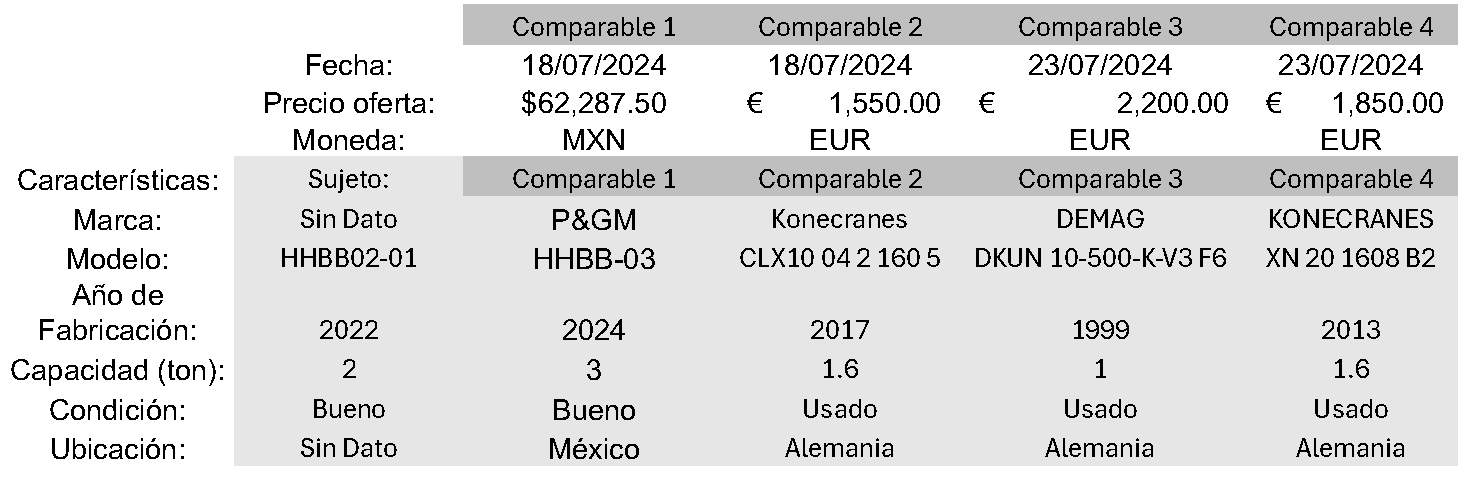
\includegraphics[width=  0.7\linewidth, page = 1]{../0.imagenes/CAP_8/mercado_2_1}
\end{figure}
\begin{figure}[hbtp!]
	\centering
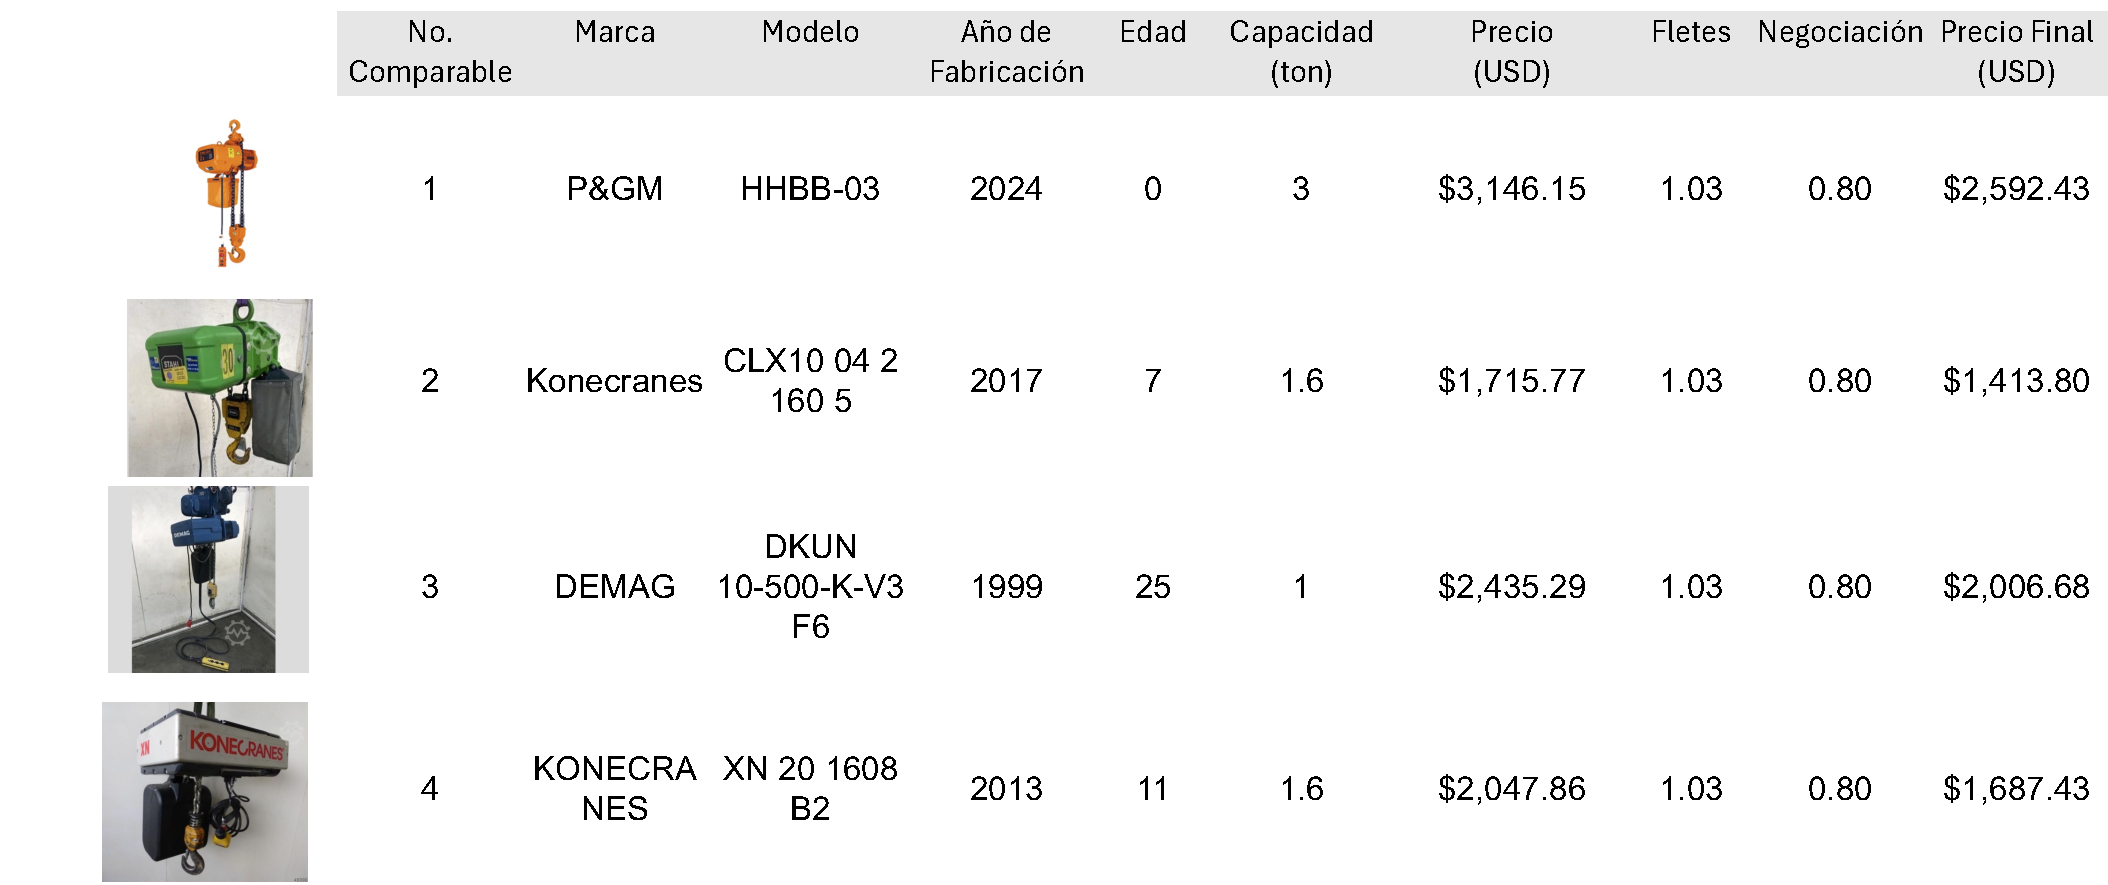
\includegraphics[width=  \linewidth, page = 1]{../0.imagenes/CAP_8/mercado_2_2}
\end{figure}
% )))

\subsection{\centering --- Variables ---} % (((
\begin{center}
  \begin{tabular}{|l|l|l|}
    \hline 
    Variable & Descripción   & Unidades\\ \hline 
    Y:  & Precio Final del activo  & USD \\ \hline 
    X1: & Edad del activo    & Años \\ \hline 
		X2: & Toneladas de cap.  & \(1000kg\) \\ \hline 
  \end{tabular}
\end{center} 
% )))

\subsection{\centering --- Matriz de Dispersion ---} % (((
\begin{center}
  \begin{tabular}{|p{11cm}|p{5cm}|}
    \hline
    Gráfica & Interpretación. \\ \hline 
    \begin{minipage}{\textwidth}
    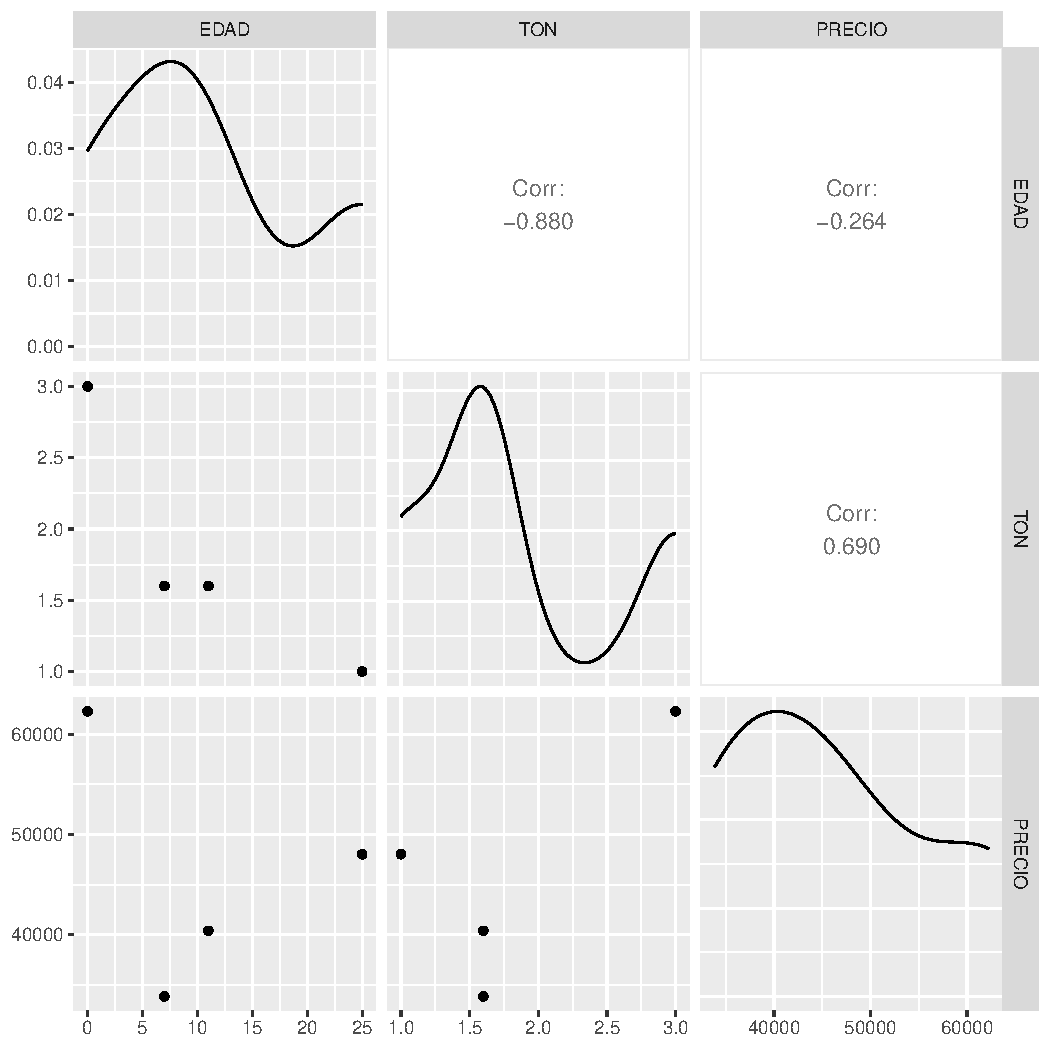
\includegraphics[width= 0.5 \linewidth, page=1]{../0.documentos/3_MERGED_MARKET/2_POLIPASTO/r/Rplots.pdf}
    \end{minipage} 
    &
		Se tiene una correlación lineal negativa fuerte (el \(88.0\%\) de los datos lo corroboran),
		entre las Toneladas de Cap. del Activo, y el Precio del Activo.
		\\ \hline 
  \end{tabular}
\end{center} 
% )))

\subsection{\centering --- Supuestos del Modelo de Regresión ---} % (((

Se realiza el análisis estadístico con un \(90\%\) de confianza. \\ 
Es decir, \(1- \alpha = 0.9\).

\subsubsection{--- Homocedasticidad ---} % (((
\begin{center}
  \begin{tabular}{|l|p{8cm}|}
    \cline{1-2}
    \multicolumn{2}{|c|}{Hipótesis}\\ \cline{1-2}
    \multicolumn{2}{|l|}{\(H_0:\) La varianza de los residuales es constante.} \\ 
    \multicolumn{2}{|l|}{\(H_a:\) La varianza de los residuales no es constante.} \\ \cline{1-2}
    Estadístico de Prueba & \(BP = 1.5527\).\\ \cline{1-2} 
		Región de Rechazo de \(H_0\) & \((0, \alpha )\).\\ \cline{1-2} 
    Valor \(p\) & \(0.4601\).\\ \cline{1-2} 
    Conclusión & Se tiene que \(p> \alpha\). \newline 
		Por tanto no se rechaza \(H_0\). \newline 
		Es decir, la varianza no es constante. \\ \cline{1-2} 
  \end{tabular}
\end{center}
% )))

\subsubsection{--- Independencia ---} % (((
\begin{center}
  \begin{tabular}{|l|p{8cm}|}
    \cline{1-2}
    \multicolumn{2}{|c|}{Hipótesis}\\ \cline{1-2}
    \multicolumn{2}{|l|}{\(H_0:\) Los residuos son independientes.} \\ 
    \multicolumn{2}{|l|}{\(H_a:\) Los residuos no son indpendientes.} \\ \cline{1-2}
    Estadístico de Prueba & \(DW = 1.3517\).\\ \cline{1-2} 
		Región de Rechazo de \(H_0\) & \((0, \alpha )\).\\ \cline{1-2} 
    Valor \(p\) & \(1\).\\ \cline{1-2} 
    Conclusión & Se tiene que \(p> \alpha\). \newline 
		Por tanto no se rechaza \(H_0\). \newline 
		Es decir, los residuos son independientes.\\ \cline{1-2} 
  \end{tabular}
\end{center}
% )))

\subsubsection{--- Normalidad ---} % (((
\begin{center}
  \begin{tabular}{|l|p{8cm}|}
    \cline{1-2}
    \multicolumn{2}{|c|}{Hipótesis}\\ \cline{1-2}
    \multicolumn{2}{|l|}{\(H_0:\) Los residuos siguen una distribución normal} \\ 
    \multicolumn{2}{|l|}{\(H_a:\) Los residuos no siguen una distribución normal.} \\ \cline{1-2}
    Estadístico de Prueba & \(W = 0.88264\).\\ \cline{1-2} 
		Región de Rechazo de \(H_0\) & \((0, \alpha )\).\\ \cline{1-2} 
    Valor \(p\) & \(0.35\).\\ \cline{1-2} 
    Conclusión & Se tiene que \(p> \alpha\). \newline 
		Por tanto no se rechaza \(H_0\). \newline 
		Es decir, los residuos siguen una distribución normal.\\ \cline{1-2} 
  \end{tabular}
\end{center}
% )))

% )))

\subsection{\centering --- Modelo de Regresión Estimado ---} % (((
\begin{align}
	Y & = &              -1,054.27 & + 73.69 \cdot X_1           & + 1,215.07   \cdot X_2   \\[2mm]
	\mbox{Precio} & = &  -1,054.27 & + 73.69 \cdot (\mbox{Edad}) & + 1,215.07   \cdot (\mbox{Ton})
	\label{eq:2}
\end{align}
% )))

\subsection{\centering --- Tabla Anova ---} % (((
\begin{center}
  \begin{tabular}{|l|l|l|l|l|}
    \hline 
    Fuentes de Variación  & Suma de Cuadrados & Grados de Libertad & Cuadrados Medios & F\\ \hline 
		Regresión & 769,648.8568  & 2 & 384,824.4284 & 1,536.308 \\ \hline
		Error     &     250.4865  & 1 &     250.4865 &    0 \\ \hline
		Totales   & 769,899.3433  & 3 & 385,074.9149 &    0 \\ \hline
  \end{tabular}
\end{center} 
% )))

\subsection{\centering --- Prueba de Significancia del Modelo ---} % (((
Se comprueba la significancia del modelo con el estadístico \(F\) de la Tabla Anova.
\begin{center}
  \begin{tabular}{|l|p{6cm}|}
    \cline{1-2}
    \multicolumn{2}{|c|}{Hipótesis}\\ \cline{1-2}
    \multicolumn{2}{|l|}{\(H_0:\) El modelo no es significativo.} \\ 
    \multicolumn{2}{|l|}{\(H_a:\) El modelo es significativo.} \\ \cline{1-2}
    Estadístico de Prueba & \(1536\).\\ \cline{1-2} 
		Región de Rechazo de \(H_0\) & \((0, \alpha )\).\\ \cline{1-2} 
    Valor \(p\) & \(0.01804\).\\ \cline{1-2} 
    Conclusión & Se tiene que \(p<\alpha\). \newline 
		Por tanto se rechaza \(H_0\). \newline 
		Es decir, el modelo es significativo.\\ \cline{1-2} 
  \end{tabular}
\end{center} 
% )))

\subsection{\centering Estimación del Valor de Mercado aplicado al Activo.} % (((
Se obtiene el valor de mercado por medio de las características del activo y el modelo de regresión \eqref{eq:2}.
\begin{center}
  \begin{tabular}{|l|l|l|}
    \hline 
		Descripción   & Unidades  & Activo \\ \hline 
    Edad del activo    & Años      & 2      \\ \hline 
		Toneladas de cap.  & \(1000kg\) & 2   \\ \hline 
		Precio del activo   & USD       & \$ 1,523.26   \\ \hline 
  \end{tabular}
\end{center} 
Se concluye que el Polipasto Eléctrico, tiene un valor de mercado de 
\$ 1,523.26  USD.
% )))

% )))

\section{Bombo Batidor/Mezclador para Cofitería.} % (((

\subsection{\centering --- Mercado Utilizado ---} % (((
Se toma la siguiente muestra estadísticamente significativa, y se 
comprueba que lo es, en las siguientes secciones.
\begin{figure}[hbtp!]
	\centering
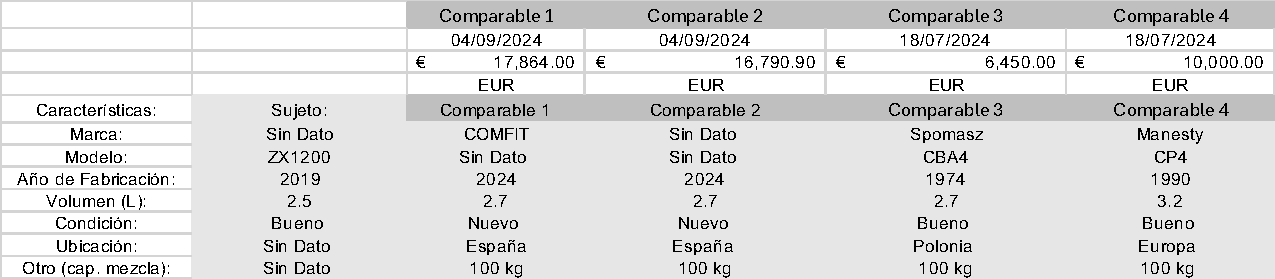
\includegraphics[width=  0.6\linewidth, page = 1]{../0.imagenes/CAP_8/mercado_3_1}
\end{figure}
\begin{figure}[hbtp!]
	\centering
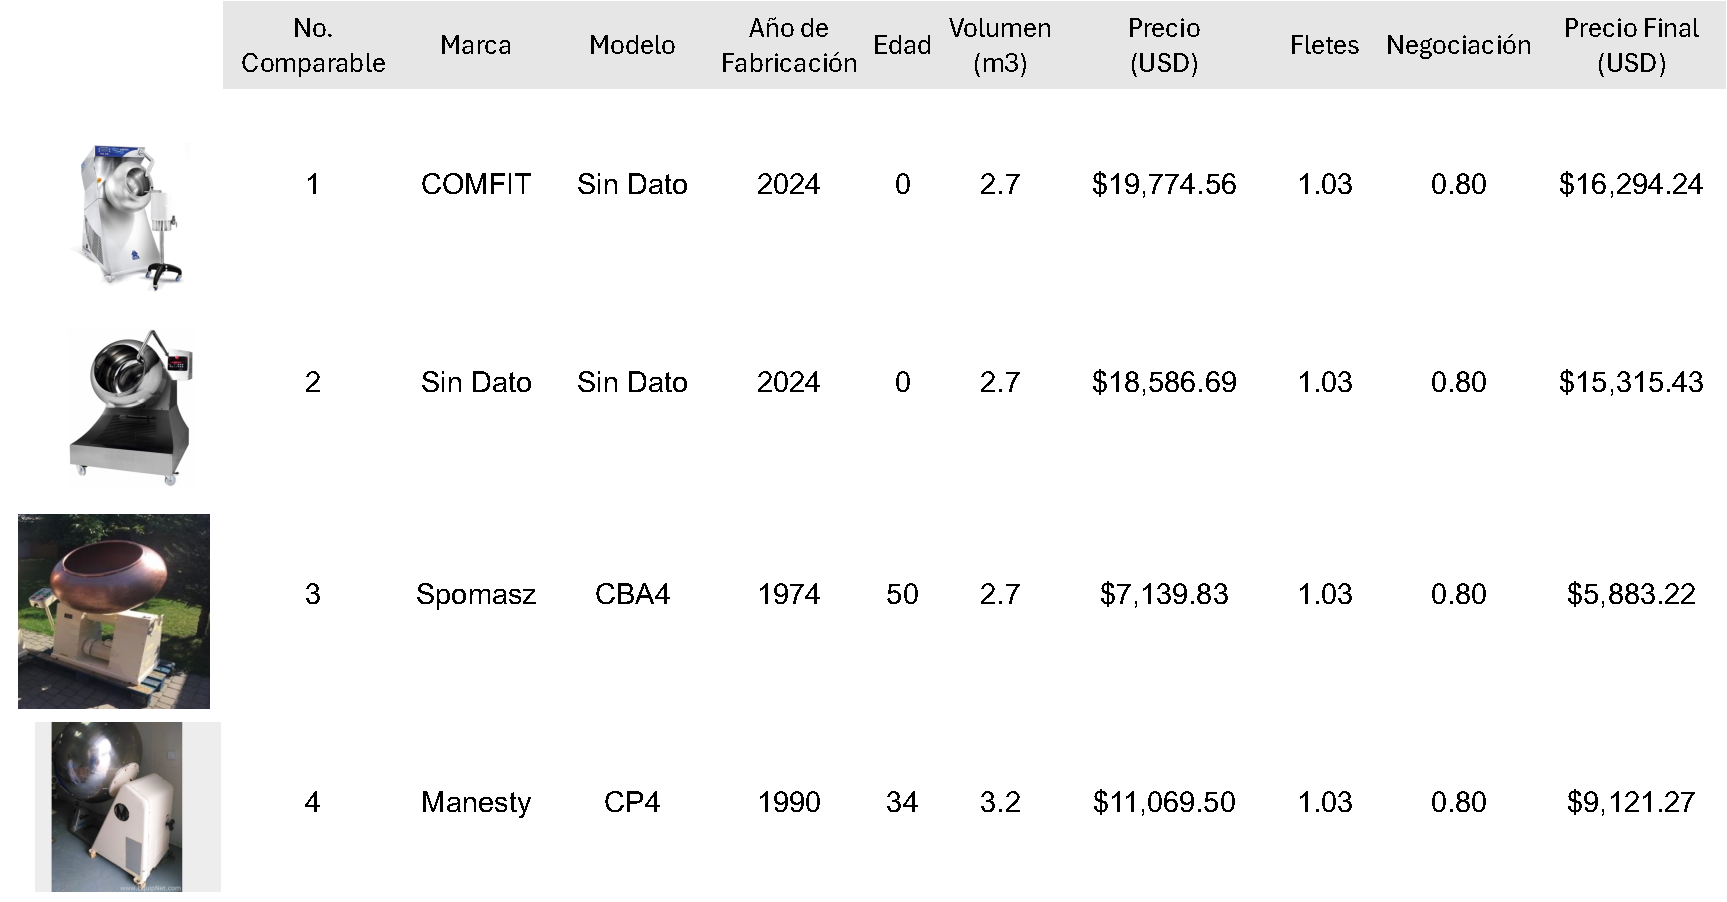
\includegraphics[width=  0.8\linewidth, page = 1]{../0.imagenes/CAP_8/mercado_3_2}
\end{figure}
% \begin{center}
	% \begin{tabular}{*{4}{|p{2cm}}|}
		% \hline 
% MARCA    & EDAD  & VOL  & PRECIO \\ \hline
% COMFIT   & 0     & 2.7  & \$38,9971.12 \\ \hline
% Sin Dato & 0     & 2.7  & \$36,6545.35 \\ \hline
% CBA4     & 50    & 2.7  & \$14,0803.50 \\ \hline
% CP4      & 34    & 3.2  & \$21,8300.00 \\ \hline
	% \end{tabular}
% \end{center}
% )))

\subsection{\centering --- Variables ---} % (((
\begin{center}
  \begin{tabular}{|l|l|l|}
    \hline 
    Variable & Descripción   & Unidades\\ \hline 
    Y:  & Precio Final del activo  & USD \\ \hline 
    X1: & Edad del activo    & Años \\ \hline 
		X2: & Volumen  & \(m ^ 3\) \\ \hline 
  \end{tabular}
\end{center} 
% )))

\subsection{\centering --- Matriz de Dispersion ---} % (((
\begin{center}
  \begin{tabular}{|p{11cm}|p{5cm}|}
    \hline
    Gráfica & Interpretación. \\ \hline 
    \begin{minipage}{\textwidth}
    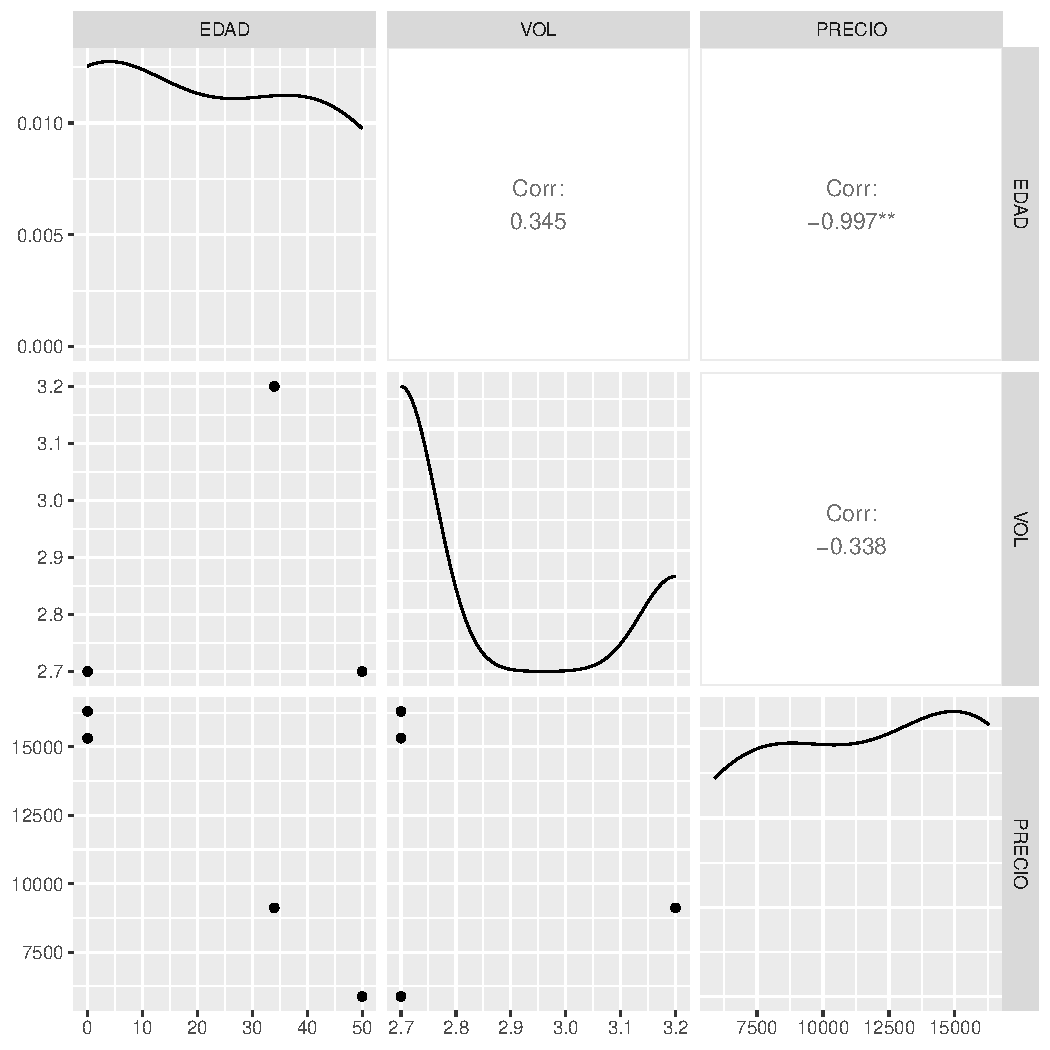
\includegraphics[width= 0.5 \linewidth, page=1]{../0.documentos/3_MERGED_MARKET/3_BOMBO_BATIDOR/r/Rplots.pdf}
    \end{minipage} 
    &
		Se tiene una correlación lineal negativa fuerte (el \(99.7\%\) de los datos lo corroboran),
		entre la Edad del Activo, y el Precio del Activo.
		\\ \hline 
  \end{tabular}
\end{center} 
% )))

\subsection{\centering --- Supuestos del Modelo de Regresión ---} % (((

Se realiza el análisis estadístico con un \(90\%\) de confianza. \\ 
Es decir, \(1- \alpha = 0.9\).

\subsubsection{--- Homocedasticidad ---} % (((
\begin{center}
  \begin{tabular}{|l|p{8cm}|}
    \cline{1-2}
    \multicolumn{2}{|c|}{Hipótesis}\\ \cline{1-2}
    \multicolumn{2}{|l|}{\(H_0:\) La varianza de los residuales es constante.} \\ 
    \multicolumn{2}{|l|}{\(H_a:\) La varianza de los residuales no es constante.} \\ \cline{1-2}
    Estadístico de Prueba & \(BP = 4\).\\ \cline{1-2} 
		Región de Rechazo de \(H_0\) & \((0, \alpha )\).\\ \cline{1-2} 
    Valor \(p\) & \(0.1353\).\\ \cline{1-2} 
    Conclusión & Se tiene que \(p> \alpha\). \newline 
		Por tanto no se rechaza \(H_0\). \newline 
		Es decir, la varianza no es constante. \\ \cline{1-2} 
  \end{tabular}
\end{center}
% )))

\subsubsection{--- Independencia ---} % (((
\begin{center}
  \begin{tabular}{|l|p{8cm}|}
    \cline{1-2}
    \multicolumn{2}{|c|}{Hipótesis}\\ \cline{1-2}
    \multicolumn{2}{|l|}{\(H_0:\) Los residuos son independientes.} \\ 
    \multicolumn{2}{|l|}{\(H_a:\) Los residuos no son indpendientes.} \\ \cline{1-2}
    Estadístico de Prueba & \(DW = 2.5\).\\ \cline{1-2} 
		Región de Rechazo de \(H_0\) & \((0, \alpha )\).\\ \cline{1-2} 
    Valor \(p\) & \(1\).\\ \cline{1-2} 
    Conclusión & Se tiene que \(p> \alpha\). \newline 
		Por tanto no se rechaza \(H_0\). \newline 
		Es decir, los residuos son independientes.\\ \cline{1-2} 
  \end{tabular}
\end{center}
% )))

\subsubsection{--- Normalidad ---} % (((
\begin{center}
  \begin{tabular}{|l|p{8cm}|}
    \cline{1-2}
    \multicolumn{2}{|c|}{Hipótesis}\\ \cline{1-2}
    \multicolumn{2}{|l|}{\(H_0:\) Los residuos siguen una distribución normal} \\ 
    \multicolumn{2}{|l|}{\(H_a:\) Los residuos no siguen una distribución normal.} \\ \cline{1-2}
    Estadístico de Prueba & \(W = 0.94466\).\\ \cline{1-2} 
		Región de Rechazo de \(H_0\) & \((0, \alpha )\).\\ \cline{1-2} 
    Valor \(p\) & \(0.683\).\\ \cline{1-2} 
    Conclusión & Se tiene que \(p> \alpha\). \newline 
		Por tanto no se rechaza \(H_0\). \newline 
		Es decir, los residuos siguen una distribución normal.\\ \cline{1-2} 
  \end{tabular}
\end{center}
% )))

% )))

\subsection{\centering --- Modelo de Regresión Estimado ---} % (((
\begin{align}
	Y & = &               15,463.91 & - 198.43 \cdot X_1           & + 126.27     \cdot X_2   \\[2mm]
	\mbox{Precio} & = &   15,463.91 & - 198.43 \cdot (\mbox{Edad}) & + 126.27     \cdot (\mbox{Volumen})
	\label{eq:3}
\end{align}
% )))

\subsection{\centering --- Tabla Anova ---} % (((
\begin{center}
  \begin{tabular}{|l|l|l|l|l|}
    \hline 
		Fuentes de Variación  & Suma de Cuadrados & Grados de Libertad & Cuadrados Medios & F\\ \hline 
		Regresión & 74,175,484.6 & 2 & 37,087,742.3 & 77.42186 \\ \hline
		Error     &    479,034.5 & 1 &    479,034.5 &  0 \\ \hline
		Totales   & 74,654,519.1 & 3 & 37,566,776.8 &  0 \\ \hline
  \end{tabular}
\end{center} 
% )))

\subsection{\centering --- Prueba de Significancia del Modelo ---} % (((
Se comprueba la significancia del modelo con el estadístico \(F\) de la Tabla Anova.
\begin{center}
  \begin{tabular}{|l|p{6cm}|}
    \cline{1-2}
    \multicolumn{2}{|c|}{Hipótesis}\\ \cline{1-2}
    \multicolumn{2}{|l|}{\(H_0:\) El modelo no es significativo.} \\ 
    \multicolumn{2}{|l|}{\(H_a:\) El modelo es significativo.} \\ \cline{1-2}
    Estadístico de Prueba & \(77.42\).\\ \cline{1-2} 
		Región de Rechazo de \(H_0\) & \((0, \alpha )\).\\ \cline{1-2} 
    Valor \(p\) & \(0.0801\).\\ \cline{1-2} 
    Conclusión & Se tiene que \(p<\alpha\). \newline 
		Por tanto se rechaza \(H_0\). \newline 
		Es decir, el modelo es significativo.\\ \cline{1-2} 
  \end{tabular}
\end{center} 
% )))

\subsection{\centering Estimación del Valor de Mercado aplicado al Activo.} % (((
Se obtiene el valor de mercado por medio de las características del activo y el modelo de regresión \eqref{eq:3}.
\begin{center}
  \begin{tabular}{|l|l|l|}
    \hline 
		Descripción   & Unidades  & Activo \\ \hline 
    Edad del activo    & Años      & 5      \\ \hline 
		Volumen  & \(m ^ 3\) & 2.5   \\ \hline 
		Precio del activo   & USD       & \$ 14,821.52  \\ \hline 
  \end{tabular}
\end{center} 
Se concluye que el Bombo Batidor/Mezclador para Confitería, tiene un valor de mercado de 
\$ 14,821.52  USD.
% )))

% )))

\section{Compresor Horizontal Oil-Free.} % (((

\subsection{\centering --- Mercado Utilizado ---} % (((
Se toma la siguiente muestra estadísticamente significativa, y se 
comprueba que lo es, en las siguientes secciones.
% \begin{figure}[hbtp!]
	% \centering
% \end{figure}
\begin{center}
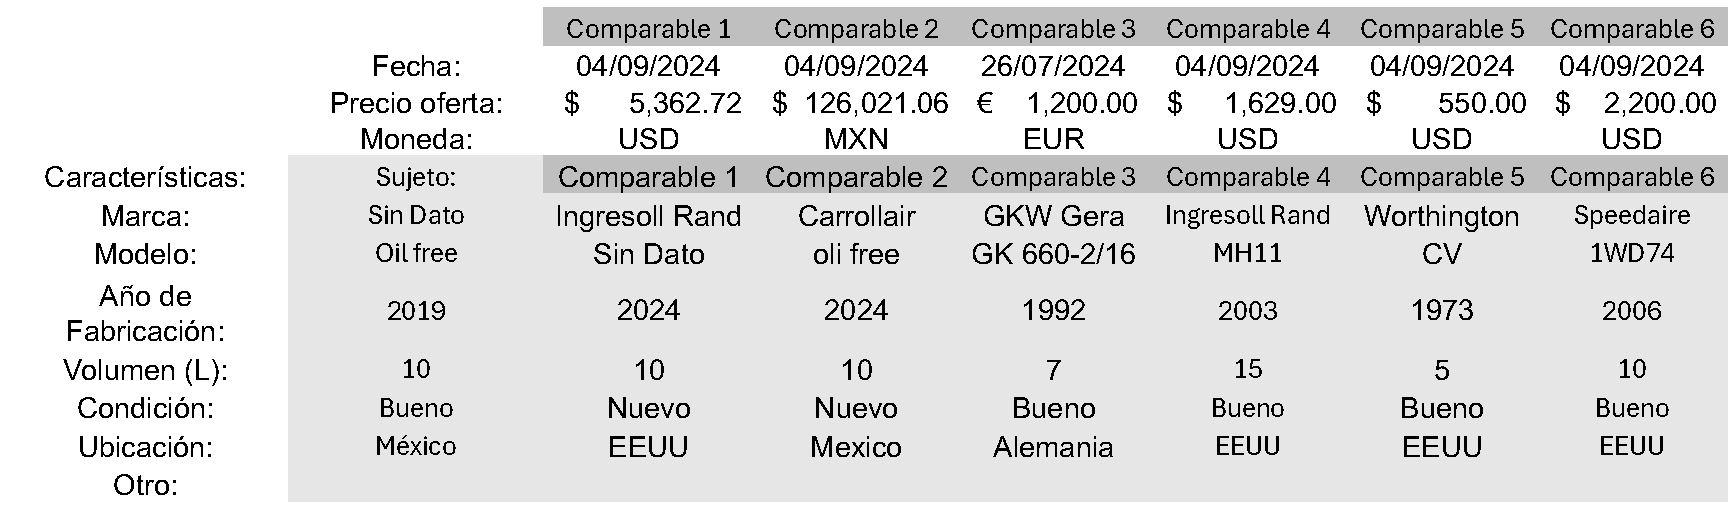
\includegraphics[width=  0.7 \linewidth, page = 1]{../0.imagenes/CAP_8/mercado_4_1}
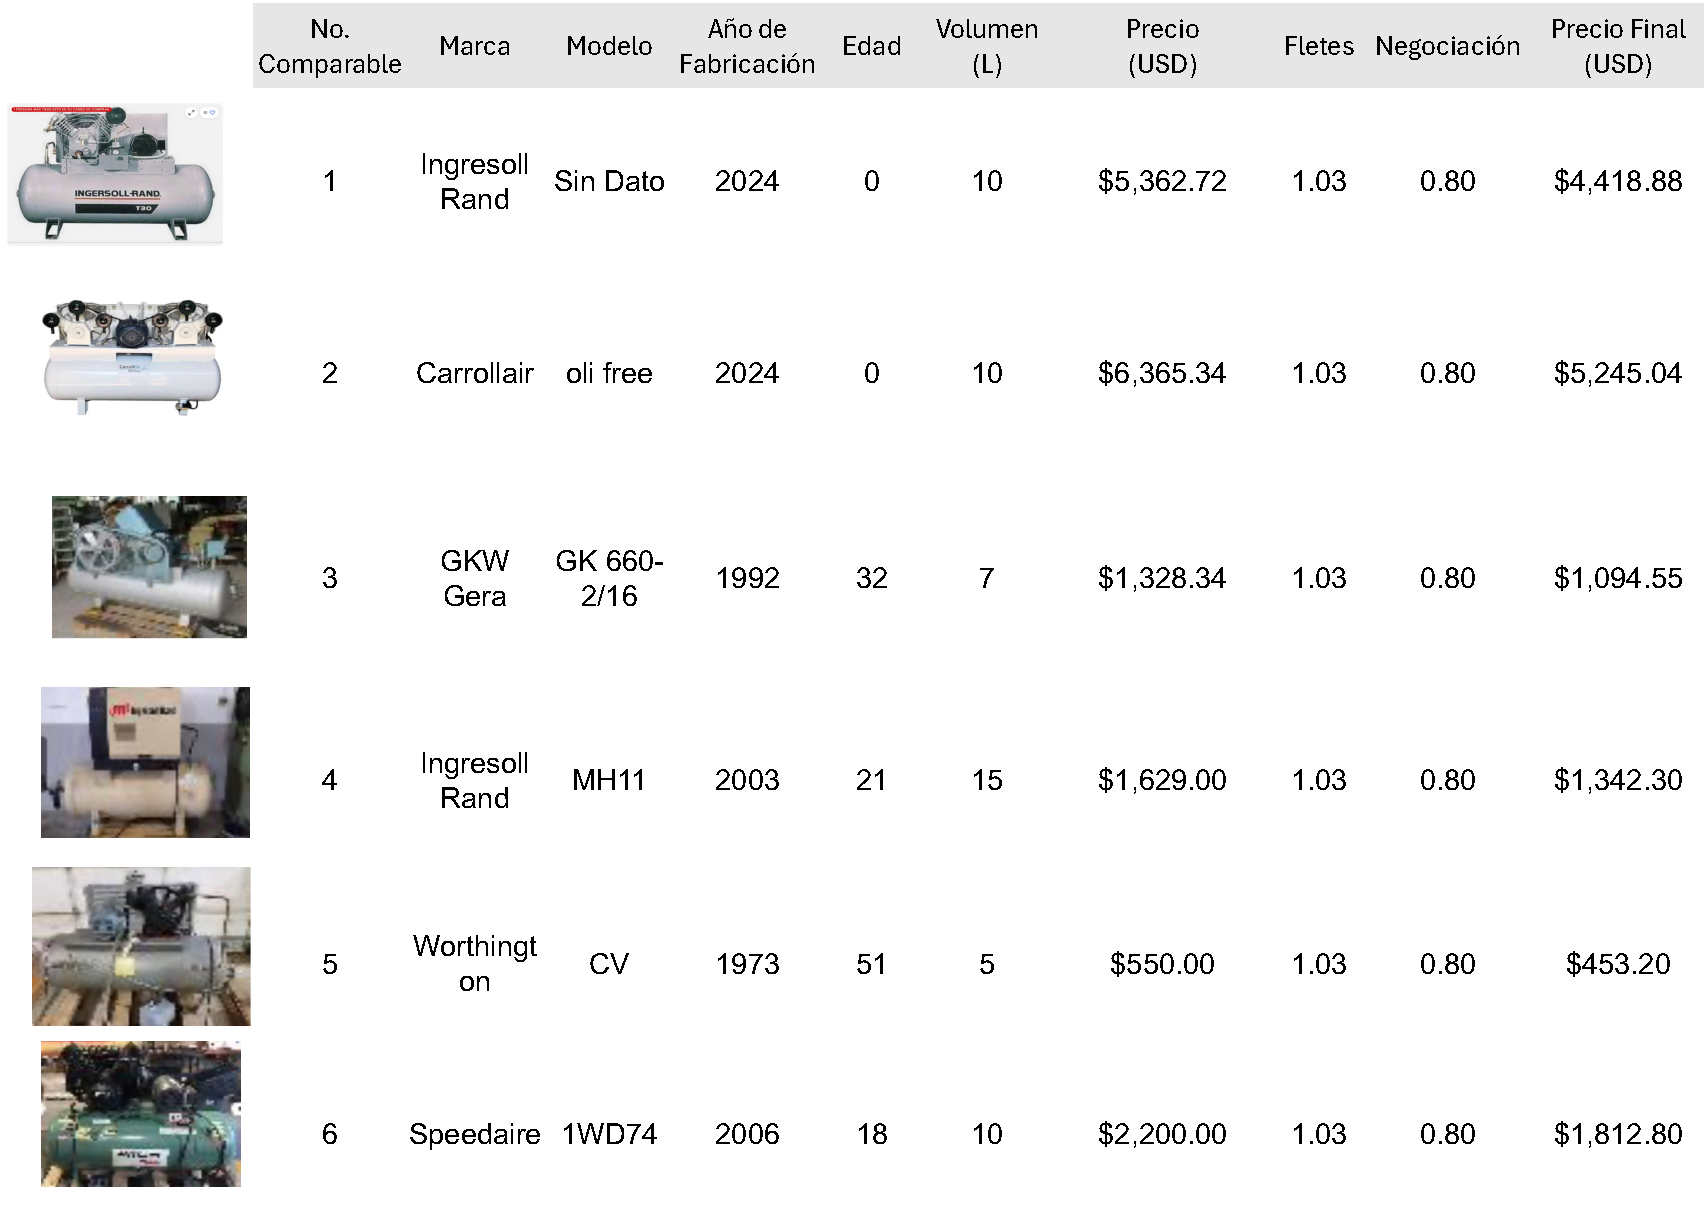
\includegraphics[width=  0.8\linewidth, page = 1]{../0.imagenes/CAP_8/mercado_4_2}
\end{center}
% )))

\subsection{\centering --- Variables ---} % (((
\begin{center}
  \begin{tabular}{|l|l|l|}
    \hline 
    Variable & Descripción   & Unidades\\ \hline 
    Y:  & Precio Final del activo  & USD \\ \hline 
    X1: & Edad del activo    & Años \\ \hline 
		X2: & Capacidad  & \(hp\) \\ \hline 
  \end{tabular}
\end{center} 
% )))

\subsection{\centering --- Matriz de Dispersion ---} % (((
\begin{center}
  \begin{tabular}{|p{11cm}|p{5cm}|}
    \hline
    Gráfica & Interpretación. \\ \hline 
    \begin{minipage}{\textwidth}
    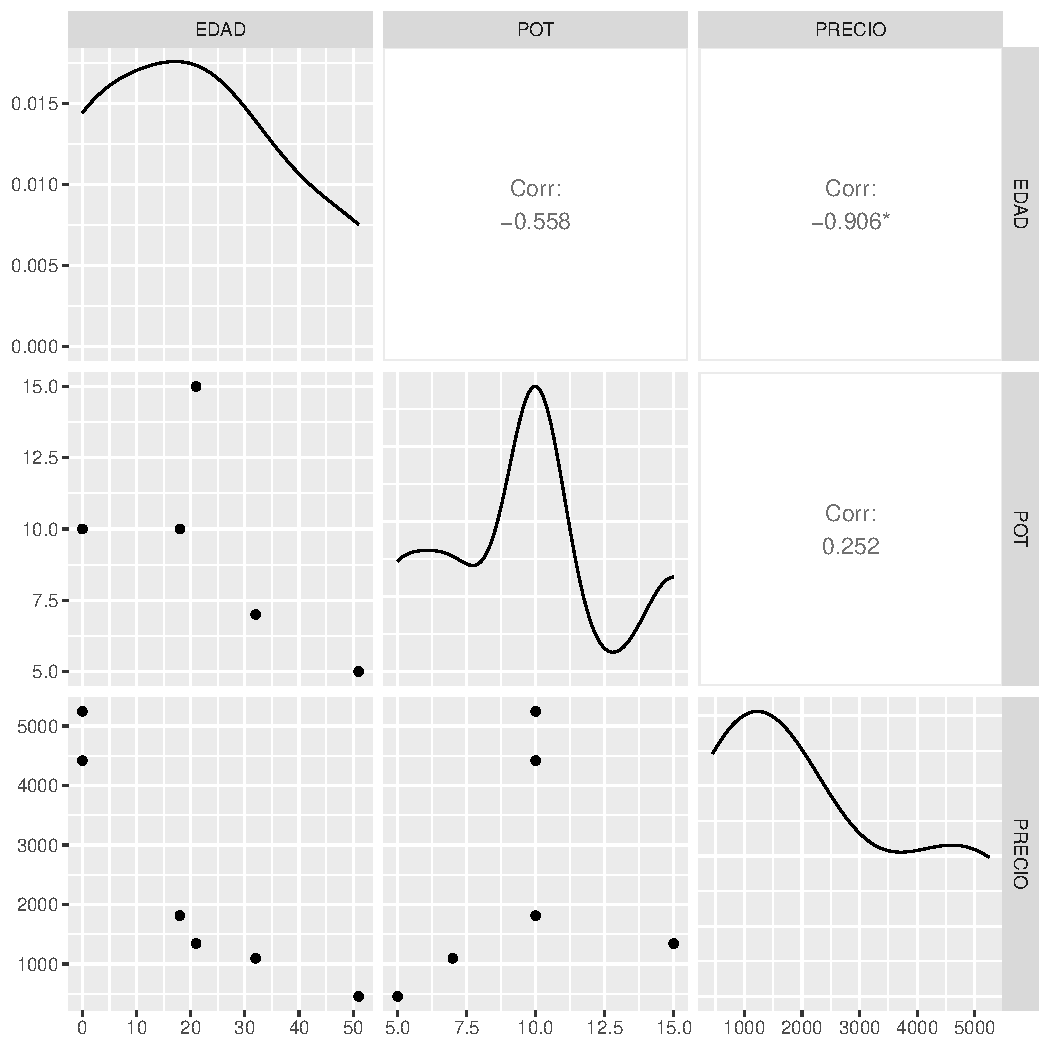
\includegraphics[width= 0.5 \linewidth, page=1]{../0.documentos/3_MERGED_MARKET/4_COMPRESOR_AIRE_OIL_FREE/r/Rplots.pdf}
    \end{minipage} 
    &
		Se tiene una correlación lineal negativa fuerte (el \(90.6\%\) de los datos lo corroboran),
		entre la Edad del Activo, y el Precio del Activo.
		\\ \hline 
  \end{tabular}
\end{center} 
% )))

\subsection{\centering --- Supuestos del Modelo de Regresión ---} % (((

Se realiza el análisis estadístico con un \(90\%\) de confianza. \\ 
Es decir, \(1- \alpha = 0.9\).

\subsubsection{--- Homocedasticidad ---} % (((
\begin{center}
  \begin{tabular}{|l|p{8cm}|}
    \cline{1-2}
    \multicolumn{2}{|c|}{Hipótesis}\\ \cline{1-2}
    \multicolumn{2}{|l|}{\(H_0:\) La varianza de los residuales es constante.} \\ 
    \multicolumn{2}{|l|}{\(H_a:\) La varianza de los residuales no es constante.} \\ \cline{1-2}
    Estadístico de Prueba & \(BP = 0.88125\).\\ \cline{1-2} 
		Región de Rechazo de \(H_0\) & \((0, \alpha )\).\\ \cline{1-2} 
    Valor \(p\) & \(0.6436\).\\ \cline{1-2} 
    Conclusión & Se tiene que \(p> \alpha\). \newline 
		Por tanto no se rechaza \(H_0\). \newline 
		Es decir, la varianza no es constante. \\ \cline{1-2} 
  \end{tabular}
\end{center}
% )))

\subsubsection{--- Independencia ---} % (((
\begin{center}
  \begin{tabular}{|l|p{8cm}|}
    \cline{1-2}
    \multicolumn{2}{|c|}{Hipótesis}\\ \cline{1-2}
    \multicolumn{2}{|l|}{\(H_0:\) Los residuos son independientes.} \\ 
    \multicolumn{2}{|l|}{\(H_a:\) Los residuos no son indpendientes.} \\ \cline{1-2}
    Estadístico de Prueba & \(DW = 2.6952\).\\ \cline{1-2} 
		Región de Rechazo de \(H_0\) & \((0, \alpha )\).\\ \cline{1-2} 
    Valor \(p\) & \(0.8627\).\\ \cline{1-2} 
    Conclusión & Se tiene que \(p> \alpha\). \newline 
		Por tanto no se rechaza \(H_0\). \newline 
		Es decir, los residuos son independientes.\\ \cline{1-2} 
  \end{tabular}
\end{center}
% )))

\subsubsection{--- Normalidad ---} % (((
\begin{center}
  \begin{tabular}{|l|p{8cm}|}
    \cline{1-2}
    \multicolumn{2}{|c|}{Hipótesis}\\ \cline{1-2}
    \multicolumn{2}{|l|}{\(H_0:\) Los residuos siguen una distribución normal} \\ 
    \multicolumn{2}{|l|}{\(H_a:\) Los residuos no siguen una distribución normal.} \\ \cline{1-2}
    Estadístico de Prueba & \(W = 0.948\).\\ \cline{1-2} 
		Región de Rechazo de \(H_0\) & \((0, \alpha )\).\\ \cline{1-2} 
    Valor \(p\) & \(0.7241\).\\ \cline{1-2} 
    Conclusión & Se tiene que \(p> \alpha\). \newline 
		Por tanto no se rechaza \(H_0\). \newline 
		Es decir, los residuos siguen una distribución normal.\\ \cline{1-2} 
  \end{tabular}
\end{center}
% )))

% )))

\subsection{\centering --- Modelo de Regresión Estimado ---} % (((
\begin{align}
	Y & = &              6,682.49 & - 111.34 \cdot X_1           & - 213.06     \cdot X_2   \\[2mm]
	\mbox{Precio} & = &  6,682.49 & - 111.34 \cdot (\mbox{Edad}) & - 213.06     \cdot (\mbox{hp})
	\label{eq:4}
\end{align}
% )))

\subsection{\centering --- Tabla Anova ---} % (((
\begin{center}
  \begin{tabular}{|l|l|l|l|l|}
    \hline 
    Fuentes de Variación  & Suma de Cuadrados & Grados de Libertad & Cuadrados Medios & F\\ \hline 
		Regresión & 17,501,850 & 2 & 8,750,925.1 & 16.15226 \\ \hline
		Error     &  1,625,332 & 3 &   541,777.3 &  0 \\ \hline
		Totales   & 19,127,182 & 5 & 9,292,702.4 &  0 \\ \hline
  \end{tabular}
\end{center} 
% )))

\subsection{\centering --- Prueba de Significancia del Modelo ---} % (((
Se comprueba la significancia del modelo con el estadístico \(F\) de la Tabla Anova.
\begin{center}
  \begin{tabular}{|l|p{6cm}|}
    \cline{1-2}
    \multicolumn{2}{|c|}{Hipótesis}\\ \cline{1-2}
    \multicolumn{2}{|l|}{\(H_0:\) El modelo no es significativo.} \\ 
    \multicolumn{2}{|l|}{\(H_a:\) El modelo es significativo.} \\ \cline{1-2}
    Estadístico de Prueba & \(16.15\).\\ \cline{1-2} 
		Región de Rechazo de \(H_0\) & \((0, \alpha )\).\\ \cline{1-2} 
    Valor \(p\) & \(0.02477\).\\ \cline{1-2} 
    Conclusión & Se tiene que \(p<\alpha\). \newline 
		Por tanto se rechaza \(H_0\). \newline 
		Es decir, el modelo es significativo.\\ \cline{1-2} 
  \end{tabular}
\end{center} 
% )))

\subsection{\centering Estimación del Valor de Mercado aplicado al Activo.} % (((
Se obtiene el valor de mercado por medio de las características del activo y el modelo de regresión \eqref{eq:4}.
\begin{center}
  \begin{tabular}{|l|l|l|}
    \hline 
		Descripción   & Unidades  & Activo \\ \hline 
    Edad del activo    & Años      & 5      \\ \hline 
		Toneladas de cap.  & \(hp\) & 10   \\ \hline 
		Precio del activo   & USD       & \$ 3,785.15     \\ \hline 
  \end{tabular}
\end{center} 
Se concluye que el Compresor Horizontal Oil-Free, tiene un valor de mercado de 
\$ 3,785.15  USD.
% )))

% )))

\section{Secador de Aire, Tipo Refrigerado.} % (((

\subsection{\centering --- Mercado Utilizado ---} % (((
Se toma la siguiente muestra estadísticamente significativa, y se 
comprueba que lo es, en las siguientes secciones.
\begin{center}
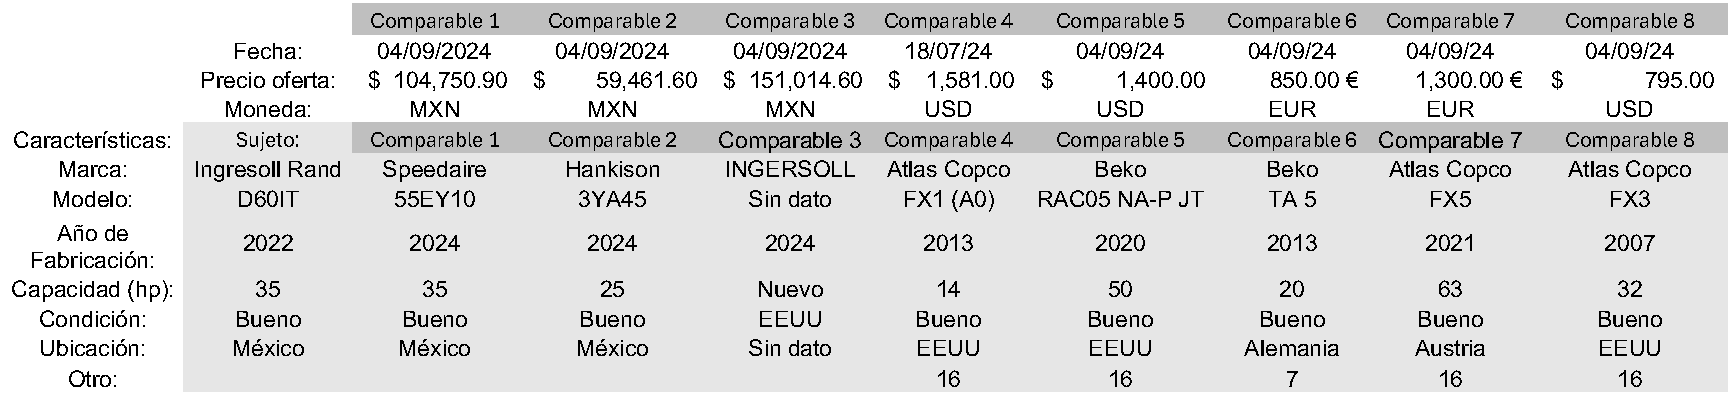
\includegraphics[width=  0.9 \linewidth, page = 1]{../0.imagenes/CAP_8/mercado_5_1}
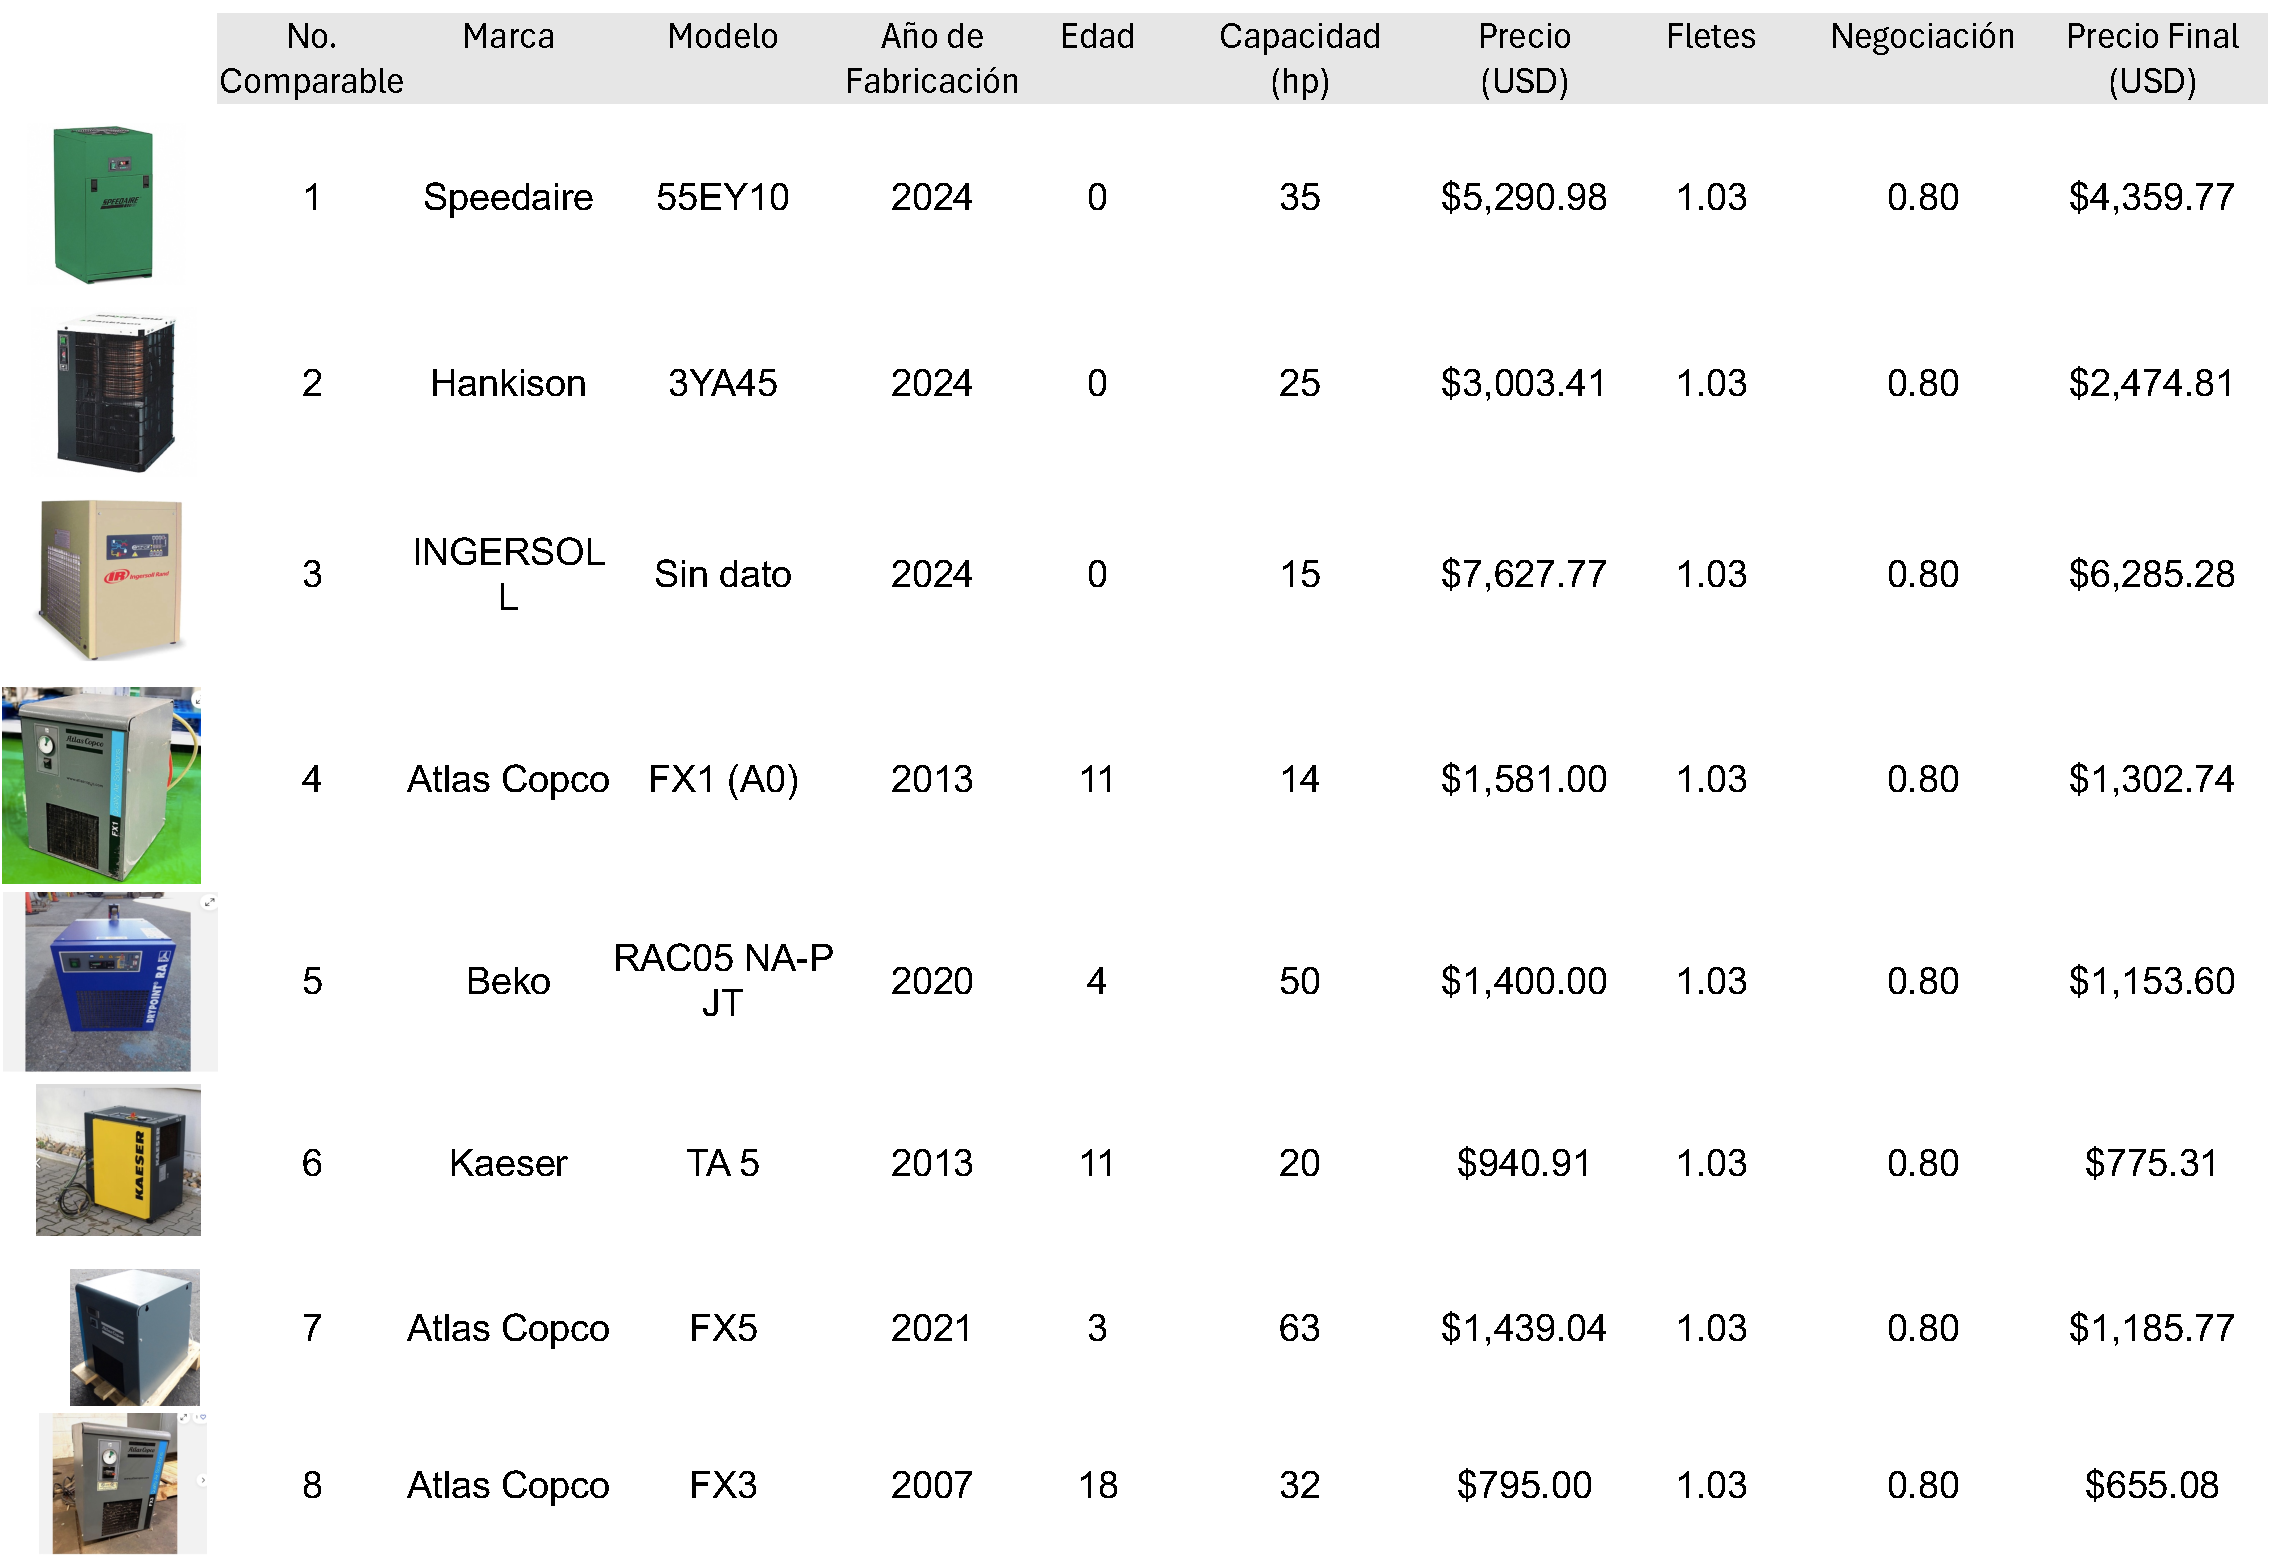
\includegraphics[width=  0.9\linewidth, page = 1]{../0.imagenes/CAP_8/mercado_5_2}
\end{center}
% )))

\subsection{\centering --- Variables ---} % (((
\begin{center}
  \begin{tabular}{|l|l|l|}
    \hline 
    Variable & Descripción   & Unidades\\ \hline 
    Y:  & Precio Final del activo  & USD \\ \hline 
    X1: & Edad del activo    & Años \\ \hline 
		X2: & Capacidad & \(hp\) \\ \hline 
  \end{tabular}
\end{center} 
% )))

\subsection{\centering --- Matriz de Dispersion ---} % (((
\begin{center}
  \begin{tabular}{|p{11cm}|p{5cm}|}
    \hline
    Gráfica & Interpretación. \\ \hline 
    \begin{minipage}{\textwidth}
    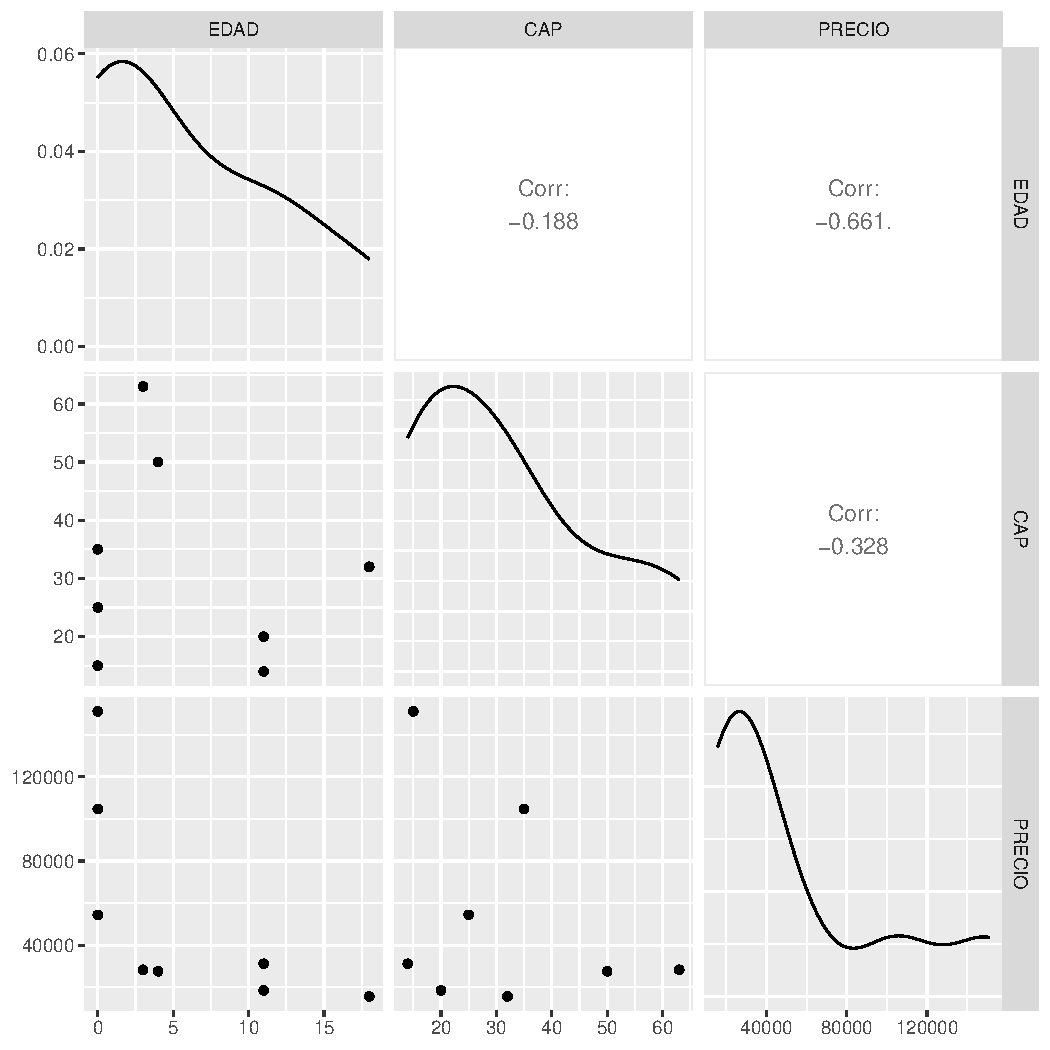
\includegraphics[width= 0.5 \linewidth, page=1]{../0.documentos/3_MERGED_MARKET/5_SECADOR_AIRE/r/Rplots.pdf}
    \end{minipage} 
    &
		Hay una correlación lineal débil (el \(66.1\%\) de los datos lo confirman),
		entre la Edad y el Precio del activo.
		\\ \hline 
  \end{tabular}
\end{center} 
% )))

\subsection{\centering --- Supuestos del Modelo de Regresión ---} % (((

Se realiza el análisis estadístico con un \(90\%\) de confianza. \\ 
Es decir, \(1- \alpha = 0.9\).

\subsubsection{--- Homocedasticidad ---} % (((
\begin{center}
  \begin{tabular}{|l|p{8cm}|}
    \cline{1-2}
    \multicolumn{2}{|c|}{Hipótesis}\\ \cline{1-2}
    \multicolumn{2}{|l|}{\(H_0:\) La varianza de los residuales es constante.} \\ 
    \multicolumn{2}{|l|}{\(H_a:\) La varianza de los residuales no es constante.} \\ \cline{1-2}
    Estadístico de Prueba & \(BP = 4.3428\).\\ \cline{1-2} 
		Región de Rechazo de \(H_0\) & \((0, \alpha )\).\\ \cline{1-2} 
    Valor \(p\) & \(0.114\).\\ \cline{1-2} 
    Conclusión & Se tiene que \(p> \alpha\). \newline 
		Por tanto no se rechaza \(H_0\). \newline 
		Es decir, la varianza no es constante. \\ \cline{1-2} 
  \end{tabular}
\end{center}
% )))

\subsubsection{--- Independencia ---} % (((
\begin{center}
  \begin{tabular}{|l|p{8cm}|}
    \cline{1-2}
    \multicolumn{2}{|c|}{Hipótesis}\\ \cline{1-2}
    \multicolumn{2}{|l|}{\(H_0:\) Los residuos son independientes.} \\ 
    \multicolumn{2}{|l|}{\(H_a:\) Los residuos no son indpendientes.} \\ \cline{1-2}
    Estadístico de Prueba & \(DW = 2.7053\).\\ \cline{1-2} 
		Región de Rechazo de \(H_0\) & \((0, \alpha )\).\\ \cline{1-2} 
    Valor \(p\) & \(0.8712\).\\ \cline{1-2} 
    Conclusión & Se tiene que \(p> \alpha\). \newline 
		Por tanto no se rechaza \(H_0\). \newline 
		Es decir, los residuos son independientes.\\ \cline{1-2} 
  \end{tabular}
\end{center}
% )))

\subsubsection{--- Normalidad ---} % (((
\begin{center}
  \begin{tabular}{|l|p{8cm}|}
    \cline{1-2}
    \multicolumn{2}{|c|}{Hipótesis}\\ \cline{1-2}
    \multicolumn{2}{|l|}{\(H_0:\) Los residuos siguen una distribución normal} \\ 
    \multicolumn{2}{|l|}{\(H_a:\) Los residuos no siguen una distribución normal.} \\ \cline{1-2}
    Estadístico de Prueba & \(W = 0.94385\).\\ \cline{1-2} 
		Región de Rechazo de \(H_0\) & \((0, \alpha )\).\\ \cline{1-2} 
    Valor \(p\) & \(0.6493\).\\ \cline{1-2} 
    Conclusión & Se tiene que \(p> \alpha\). \newline 
		Por tanto no se rechaza \(H_0\). \newline 
		Es decir, los residuos siguen una distribución normal.\\ \cline{1-2} 
  \end{tabular}
\end{center}
% )))

% )))

\subsection{\centering --- Modelo de Regresión Estimado ---} % (((
\begin{align}
	Y & = &              5,399.82 & - 230.59 \cdot X_1           & - 55.78  \cdot X_2   \\[2mm]
	\mbox{Precio} & = &  5,399.82 & - 230.59 \cdot (\mbox{Edad}) & - 55.78  \cdot (\mbox{hp})
	\label{eq:5}
\end{align}
% )))

\subsection{\centering --- Tabla Anova ---} % (((
\begin{center}
  \begin{tabular}{|l|l|l|l|l|}
    \hline 
    Fuentes de Variación  & Suma de Cuadrados & Grados de Libertad & Cuadrados Medios & F\\ \hline 
		Regresión & 19,332,765 & 2 &  9,666,383 & 5.142665 \\ \hline
		Error     &  9,398,223 & 5 &  1,879,645 & 0 \\ \hline
		Totales   & 28,730,989 & 7 & 11,546,027 & 0 \\ \hline
  \end{tabular}
\end{center} 
% )))

\subsection{\centering --- Prueba de Significancia del Modelo ---} % (((
Se comprueba la significancia del modelo con el estadístico \(F\) de la Tabla Anova.
\begin{center}
  \begin{tabular}{|l|p{6cm}|}
    \cline{1-2}
    \multicolumn{2}{|c|}{Hipótesis}\\ \cline{1-2}
    \multicolumn{2}{|l|}{\(H_0:\) El modelo no es significativo.} \\ 
    \multicolumn{2}{|l|}{\(H_a:\) El modelo es significativo.} \\ \cline{1-2}
    Estadístico de Prueba & \(5.143\).\\ \cline{1-2} 
		Región de Rechazo de \(H_0\) & \((0, \alpha )\).\\ \cline{1-2} 
    Valor \(p\) & \(0.0612\).\\ \cline{1-2} 
    Conclusión & Se tiene que \(p<\alpha\). \newline 
		Por tanto se rechaza \(H_0\). \newline 
		Es decir, el modelo es significativo.\\ \cline{1-2} 
  \end{tabular}
\end{center} 
% )))

\subsection{\centering Estimación del Valor de Mercado aplicado al Activo.} % (((
Se obtiene el valor de mercado por medio de las características del activo y el modelo de regresión \eqref{eq:5}.
\begin{center}
  \begin{tabular}{|l|l|l|}
    \hline 
		Descripción   & Unidades  & Activo \\ \hline 
    Edad del activo    & Años      & 2      \\ \hline 
		Capacidad  & \(hp\) & 35   \\ \hline 
		Precio del activo   & USD       & \$ 3,062.378  \\ \hline 
  \end{tabular}
\end{center} 
Se concluye que el Secador de Aire tipo Refrigerado, tiene un valor de mercado de 
\$ 3,062.378  USD.
% )))

% )))

\section{Compresor Tipo Tornillo.} % (((

\subsection{\centering --- Mercado Utilizado ---} % (((
Se toma la siguiente muestra estadísticamente significativa, y se 
comprueba que lo es, en las siguientes secciones.
\begin{figure}[hbtp!]
	\centering
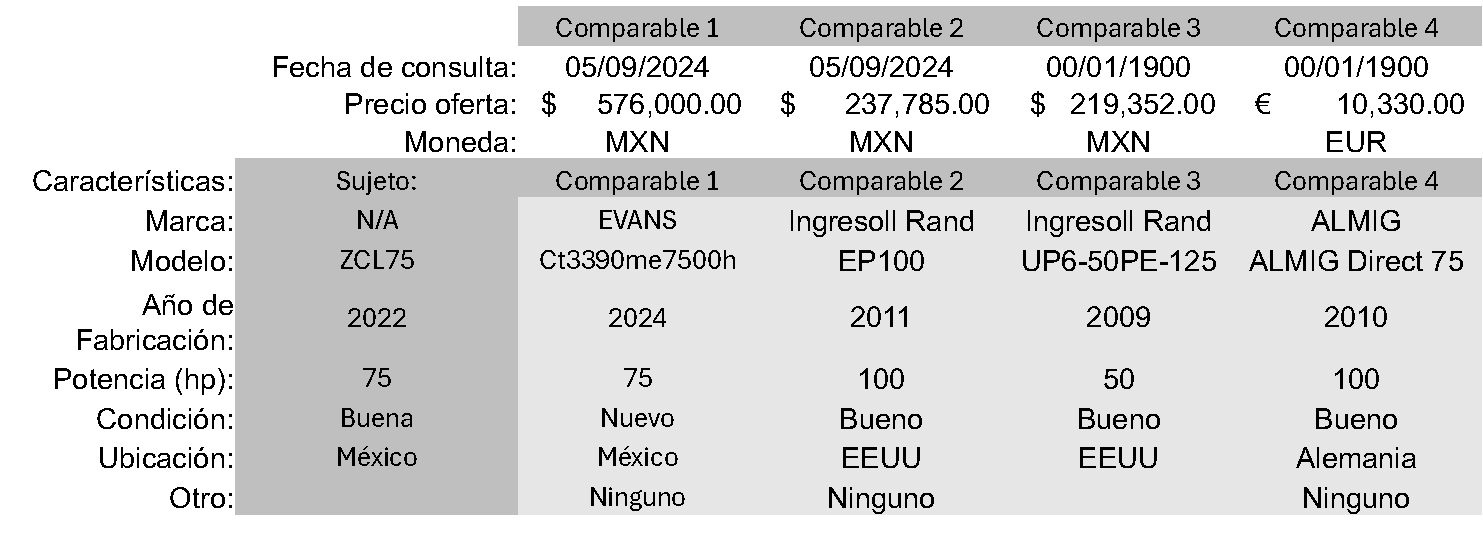
\includegraphics[width=  0.7\linewidth, page = 1]{../0.imagenes/CAP_8/mercado_6_1}
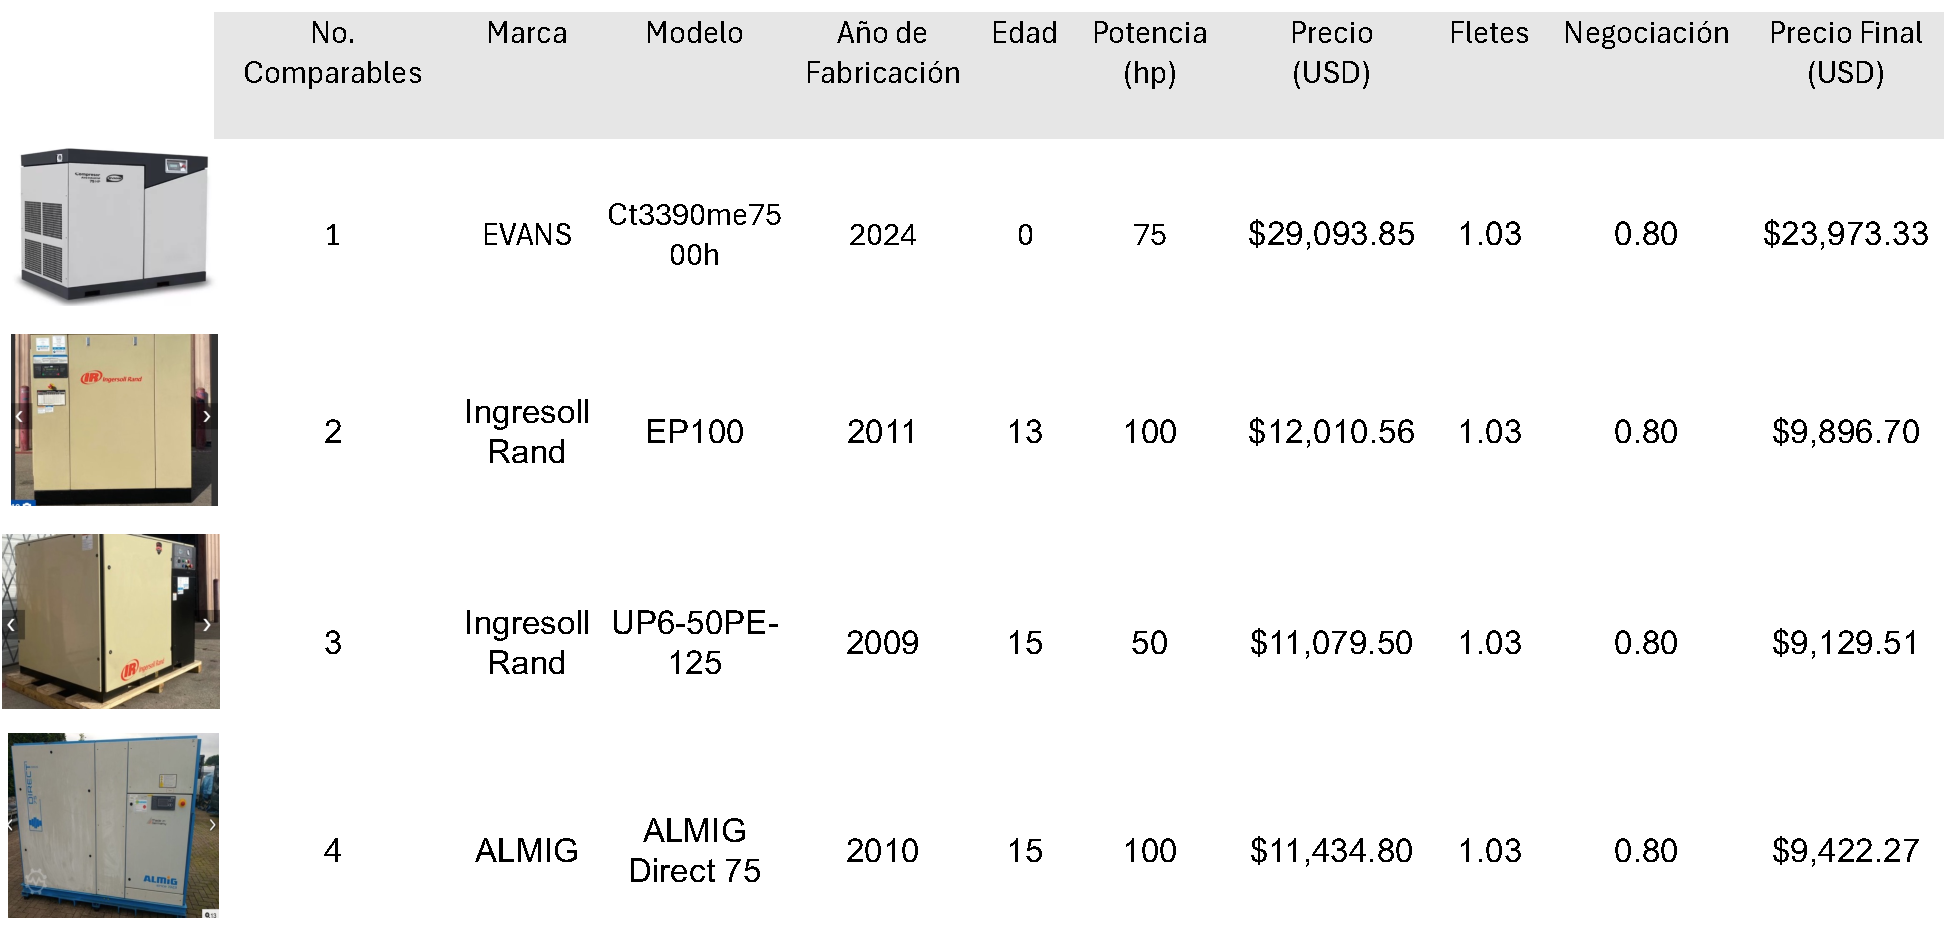
\includegraphics[width=  0.9\linewidth, page = 1]{../0.imagenes/CAP_8/mercado_6_2}
\end{figure}
% )))

\subsection{\centering --- Variables ---} % (((
\begin{center}
  \begin{tabular}{|l|l|l|}
    \hline 
    Variable & Descripción   & Unidades\\ \hline 
    Y:  & Precio Final del activo  & USD \\ \hline 
    X1: & Edad del activo    & Años \\ \hline 
		X2: & Potencia  & \(hp\) \\ \hline 
  \end{tabular}
\end{center} 
% )))

\subsection{\centering --- Matriz de Dispersion ---} % (((
\begin{center}
  \begin{tabular}{|p{11cm}|p{5cm}|}
    \hline
    Gráfica & Interpretación. \\ \hline 
    \begin{minipage}{\textwidth}
    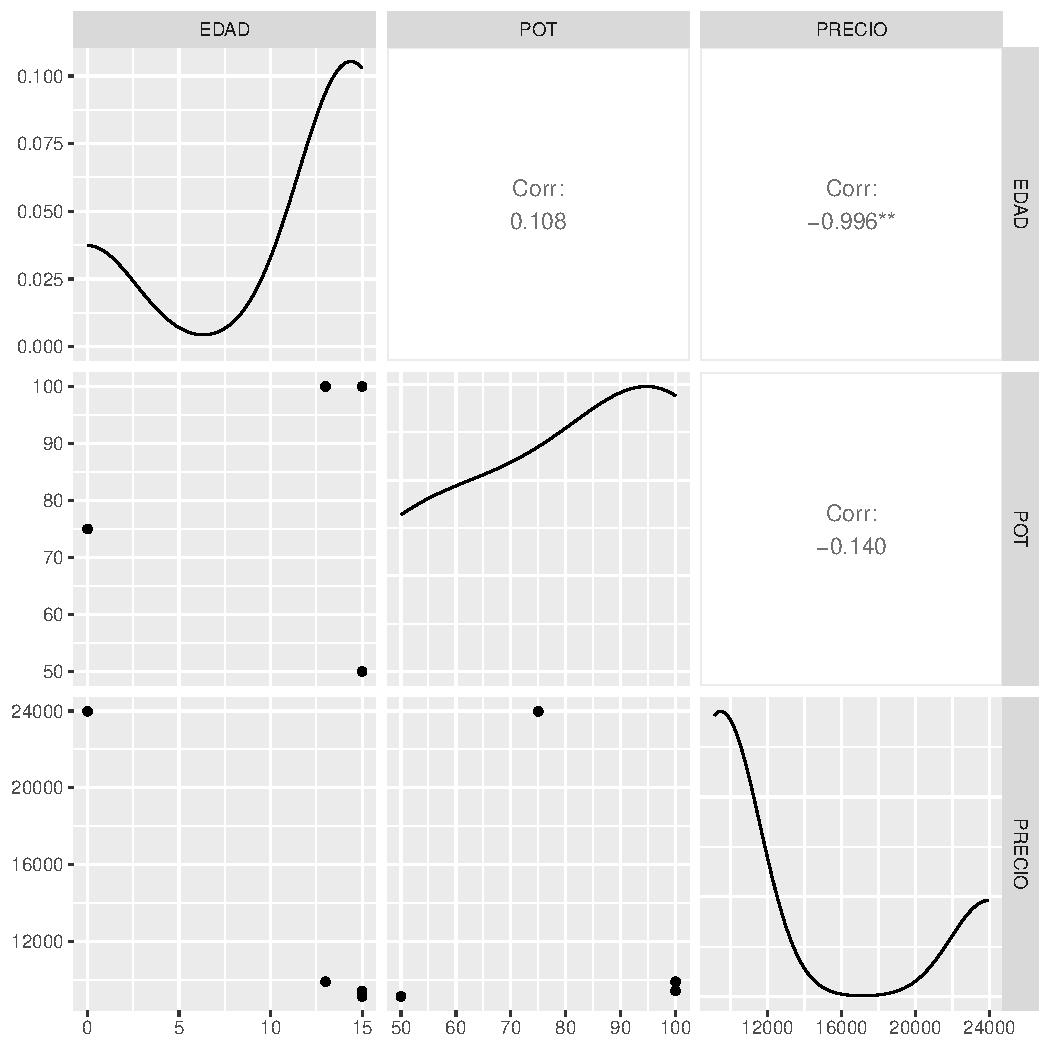
\includegraphics[width= 0.5 \linewidth, page=1]{../0.documentos/3_MERGED_MARKET/6_COMPRESOR_TIPO_TORNILLO/r/Rplots.pdf}
    \end{minipage} 
    &
		Se tiene una correlación lineal negativa fuerte (el \(99.6\%\) de los datos lo corroboran),
		entre la Edad del Activo, y el Precio del Activo.
		\\ \hline 
  \end{tabular}
\end{center} 
% )))

\subsection{\centering --- Supuestos del Modelo de Regresión ---} % (((

Se realiza el análisis estadístico con un \(90\%\) de confianza. \\ 
Es decir, \(1- \alpha = 0.9\).

\subsubsection{--- Homocedasticidad ---} % (((
\begin{center}
  \begin{tabular}{|l|p{8cm}|}
    \cline{1-2}
    \multicolumn{2}{|c|}{Hipótesis}\\ \cline{1-2}
    \multicolumn{2}{|l|}{\(H_0:\) La varianza de los residuales es constante.} \\ 
    \multicolumn{2}{|l|}{\(H_a:\) La varianza de los residuales no es constante.} \\ \cline{1-2}
    Estadístico de Prueba & \(BP = 3.9163\).\\ \cline{1-2} 
		Región de Rechazo de \(H_0\) & \((0, \alpha )\).\\ \cline{1-2} 
    Valor \(p\) & \(0.1411\).\\ \cline{1-2} 
    Conclusión & Se tiene que \(p> \alpha\). \newline 
		Por tanto no se rechaza \(H_0\). \newline 
		Es decir, la varianza no es constante. \\ \cline{1-2} 
  \end{tabular}
\end{center}
% )))

\subsubsection{--- Independencia ---} % (((
\begin{center}
  \begin{tabular}{|l|p{8cm}|}
    \cline{1-2}
    \multicolumn{2}{|c|}{Hipótesis}\\ \cline{1-2}
    \multicolumn{2}{|l|}{\(H_0:\) Los residuos son independientes.} \\ 
    \multicolumn{2}{|l|}{\(H_a:\) Los residuos no son indpendientes.} \\ \cline{1-2}
    Estadístico de Prueba & \(DW = 1.6667\).\\ \cline{1-2} 
		Región de Rechazo de \(H_0\) & \((0, \alpha )\).\\ \cline{1-2} 
    Valor \(p\) & \(1\).\\ \cline{1-2} 
    Conclusión & Se tiene que \(p> \alpha\). \newline 
		Por tanto no se rechaza \(H_0\). \newline 
		Es decir, los residuos son independientes.\\ \cline{1-2} 
  \end{tabular}
\end{center}
% )))

\subsubsection{--- Normalidad ---} % (((
\begin{center}
  \begin{tabular}{|l|p{8cm}|}
    \cline{1-2}
    \multicolumn{2}{|c|}{Hipótesis}\\ \cline{1-2}
    \multicolumn{2}{|l|}{\(H_0:\) Los residuos siguen una distribución normal} \\ 
    \multicolumn{2}{|l|}{\(H_a:\) Los residuos no siguen una distribución normal.} \\ \cline{1-2}
    Estadístico de Prueba & \(W = 0.97975\).\\ \cline{1-2} 
		Región de Rechazo de \(H_0\) & \((0, \alpha )\).\\ \cline{1-2} 
    Valor \(p\) & \(0.9005\).\\ \cline{1-2} 
    Conclusión & Se tiene que \(p> \alpha\). \newline 
		Por tanto no se rechaza \(H_0\). \newline 
		Es decir, los residuos siguen una distribución normal.\\ \cline{1-2} 
  \end{tabular}
\end{center}
% )))

% )))

\subsection{\centering --- Modelo de Regresión Estimado ---} % (((
\begin{align}
	Y & = &              24,606.27 & - 995.51 \cdot X_1           & - 9.834  \cdot X_2   \\[2mm]
	\mbox{Precio} & = &  24,606.27 & - 995.51 \cdot (\mbox{Edad}) & - 9.834  \cdot (\mbox{hp})
	\label{eq:6}
\end{align}
% )))

\subsection{\centering --- Tabla Anova ---} % (((
\begin{center}
  \begin{tabular}{|l|l|l|l|l|}
    \hline 
    Fuentes de Variación  & Suma de Cuadrados & Grados de Libertad & Cuadrados Medios & F\\ \hline 
		Regresión & 156,615,716 & 2 & 78,307,858 & 67.21184 \\ \hline
		Error     &   1,165,090 & 1 &  1,165,090 &  0 \\ \hline
		Totales   & 157,780,806 & 3 & 79,472,948 &  0 \\ \hline
  \end{tabular}
\end{center} 
% )))

\subsection{\centering --- Prueba de Significancia del Modelo ---} % (((
Se comprueba la significancia del modelo con el estadístico \(F\) de la Tabla Anova.
\begin{center}
  \begin{tabular}{|l|p{6cm}|}
    \cline{1-2}
    \multicolumn{2}{|c|}{Hipótesis}\\ \cline{1-2}
    \multicolumn{2}{|l|}{\(H_0:\) El modelo no es significativo.} \\ 
    \multicolumn{2}{|l|}{\(H_a:\) El modelo es significativo.} \\ \cline{1-2}
    Estadístico de Prueba & \(67.21\).\\ \cline{1-2} 
		Región de Rechazo de \(H_0\) & \((0, \alpha )\).\\ \cline{1-2} 
    Valor \(p\) & \(0.08593\).\\ \cline{1-2} 
    Conclusión & Se tiene que \(p<\alpha\). \newline 
		Por tanto se rechaza \(H_0\). \newline 
		Es decir, el modelo es significativo.\\ \cline{1-2} 
  \end{tabular}
\end{center} 
% )))

\subsection{\centering Estimación del Valor de Mercado aplicado al Activo.} % (((
Se obtiene el valor de mercado por medio de las características del activo y el modelo de regresión \eqref{eq:6}.
\begin{center}
  \begin{tabular}{|l|l|l|}
    \hline 
		Descripción   & Unidades  & Activo \\ \hline 
    Edad del activo    & Años      & 2      \\ \hline 
		Capacidad  & \(hp\) & 75   \\ \hline 
		Precio del activo   & USD       & \$ 21,847.12     \\ \hline 
  \end{tabular}
\end{center} 
Se concluye que el Compresor tipo Tornillo, tiene un valor de mercado de 
\$ 21,847.12  USD.
% )))

% )))

\espacio

% )))
